\documentclass[format=acmsmall, review=false, screen=true]{acmart}

\usepackage{amssymb, amsmath}
\usepackage{graphicx}
\usepackage{tikz}
\usepackage{standalone}
\usepackage{url}
\usepackage{wrapfig}
\usepackage{array}
\usepackage[inline]{enumitem}
\usepackage{footnote}
\usepackage{booktabs}
\usepackage{multirow}


% Copyright
%\setcopyright{none}
%\setcopyright{acmcopyright}
%\setcopyright{acmlicensed}
\setcopyright{rightsretained}
%\setcopyright{usgov}
%\setcopyright{usgovmixed}
%\setcopyright{cagov}
%\setcopyright{cagovmixed}

% DOI
%\acmDOI{10.475/123_4}

% ISBN
%\acmISBN{123-4567-24-567/08/06}

%Conference
\copyrightyear{2018}
\acmYear{2018}
\setcopyright{acmlicensed}
\acmConference[SIGSPATIAL '18]{26th ACM SIGSPATIAL International Conference on Advances in Geographic Information Systems}{November 6--9, 2018}{Seattle, WA, USA}
\acmBooktitle{26th ACM SIGSPATIAL International Conference on Advances in Geographic Information Systems (SIGSPATIAL '18), November 6--9, 2018, Seattle, WA, USA}
\acmPrice{15.00}
\acmDOI{10.1145/3274895.3274955}
\acmISBN{978-1-4503-5889-7/18/11}

\makesavenoteenv{table}

\newcommand{\ignore}[1]{}
\newcommand\todo[1]{\textcolor{blue}{[TODO: #1]}}
\newcommand\TODO[1]{\textcolor{blue}{\small [TODO: #1]}}

\usetikzlibrary{calc,trees,positioning,arrows,chains,shapes.geometric,%
  decorations.pathreplacing,decorations.pathmorphing,shapes,%
  decorations.text, fit, shapes.geometric, hobby, backgrounds, calc,
  matrix,shapes.symbols,plotmarks,decorations.markings,shadows}
%
\renewcommand{\topfraction}{0.96}
\renewcommand{\textfraction}{0.01}
\renewcommand{\floatpagefraction}{0.96}

\makeatletter
\DeclareRobustCommand*\cal{\@fontswitch\relax\mathcal}
\makeatother

\begin{document}

\title{Efficient Generation of Geographically Accurate Transit Maps}

\author{Hannah Bast}
\affiliation{%
  \institution{University of Freiburg}
  \city{Freiburg}
  \state{Germany}
}
\email{bast@cs.uni-freiburg.de}

\author{Patrick Brosi}
\affiliation{%
  \institution{University of Freiburg}
  \city{Freiburg}
  \state{Germany}
}
\email{brosi@cs.uni-freiburg.de}

\author{Sabine Storandt}
\affiliation{%
  \institution{JMU W\"urzburg}
  \city{W\"urzburg}
  \state{Germany}
}
\email{storandt@informatik.uni-wuerzburg.de}

\begin{abstract}
We present LOOM (Line-Ordering Optimized Maps), a fully automatic generator of geographically accurate transit maps.
The input to LOOM is data about the lines of a given transit network, namely for each line, the sequence of stations it serves and the geographical course the vehicles of this line take. We parse this data from GTFS, the prevailing standard for public transit data.
LOOM proceeds in three stages:
	(1) construct a so-called line graph, where edges correspond to segments of the network with the same set of lines following the same course;
	(2) construct an ILP that yields a line ordering for each edge which minimizes the total number of line crossings and line separations;
	(3) based on the line graph and the ILP solution, draw the map.
As a naive ILP formulation is too demanding, we derive a new custom-tailored formulation which requires significantly fewer constraints. Furthermore, we present engineering techniques which use structural properties of the line graph to further reduce the ILP size. For the subway network of New York, we can reduce the number of constraints from 229,000 in the naive ILP formulation to about 3,700 with our techniques, enabling solution times of less than a second. Since our maps respect the geography of the transit network, they can be used for tiles and overlays in typical map services. Previous research work either did not take the geographical course of the lines into account, or was concerned with schematic maps without optimizing line crossings or line separations.
\end{abstract}

\def\UrlFont{\normalsize}

%
% The code below should be generated by the tool at
% http://dl.acm.org/ccs.cfm
% Please copy and paste the code instead of the example below.
%
\begin{CCSXML}
<ccs2012>
<concept>
<concept_id>10003120.10003145.10003146.10010892</concept_id>
<concept_desc>Human-centered computing~Graph drawings</concept_desc>
<concept_significance>500</concept_significance>
</concept>
<concept>
<concept_id>10003752.10003809.10003716.10011141.10010045</concept_id>
<concept_desc>Theory of computation~Integer programming</concept_desc>
<concept_significance>500</concept_significance>
</concept>
</ccs2012>
\end{CCSXML}

\ccsdesc[500]{Human-centered computing~Graph drawings}
\ccsdesc[500]{Theory of computation~Integer programming}

\keywords{Public Transit Network, Graph Drawing, Map generation, Graphical Optimization}

\maketitle

\urlstyle{same}
\section{Introduction}\label{SEC:intro}
%

Cities with a public transit network usually have a map which illustrates the network and which is posted at all stations. Many map services also feature a transit layer where all lines and stations in an area are displayed.
Such a map should satisfy the following main criteria:\vspace{0pt}

% \begin{figure}
% \centering
% 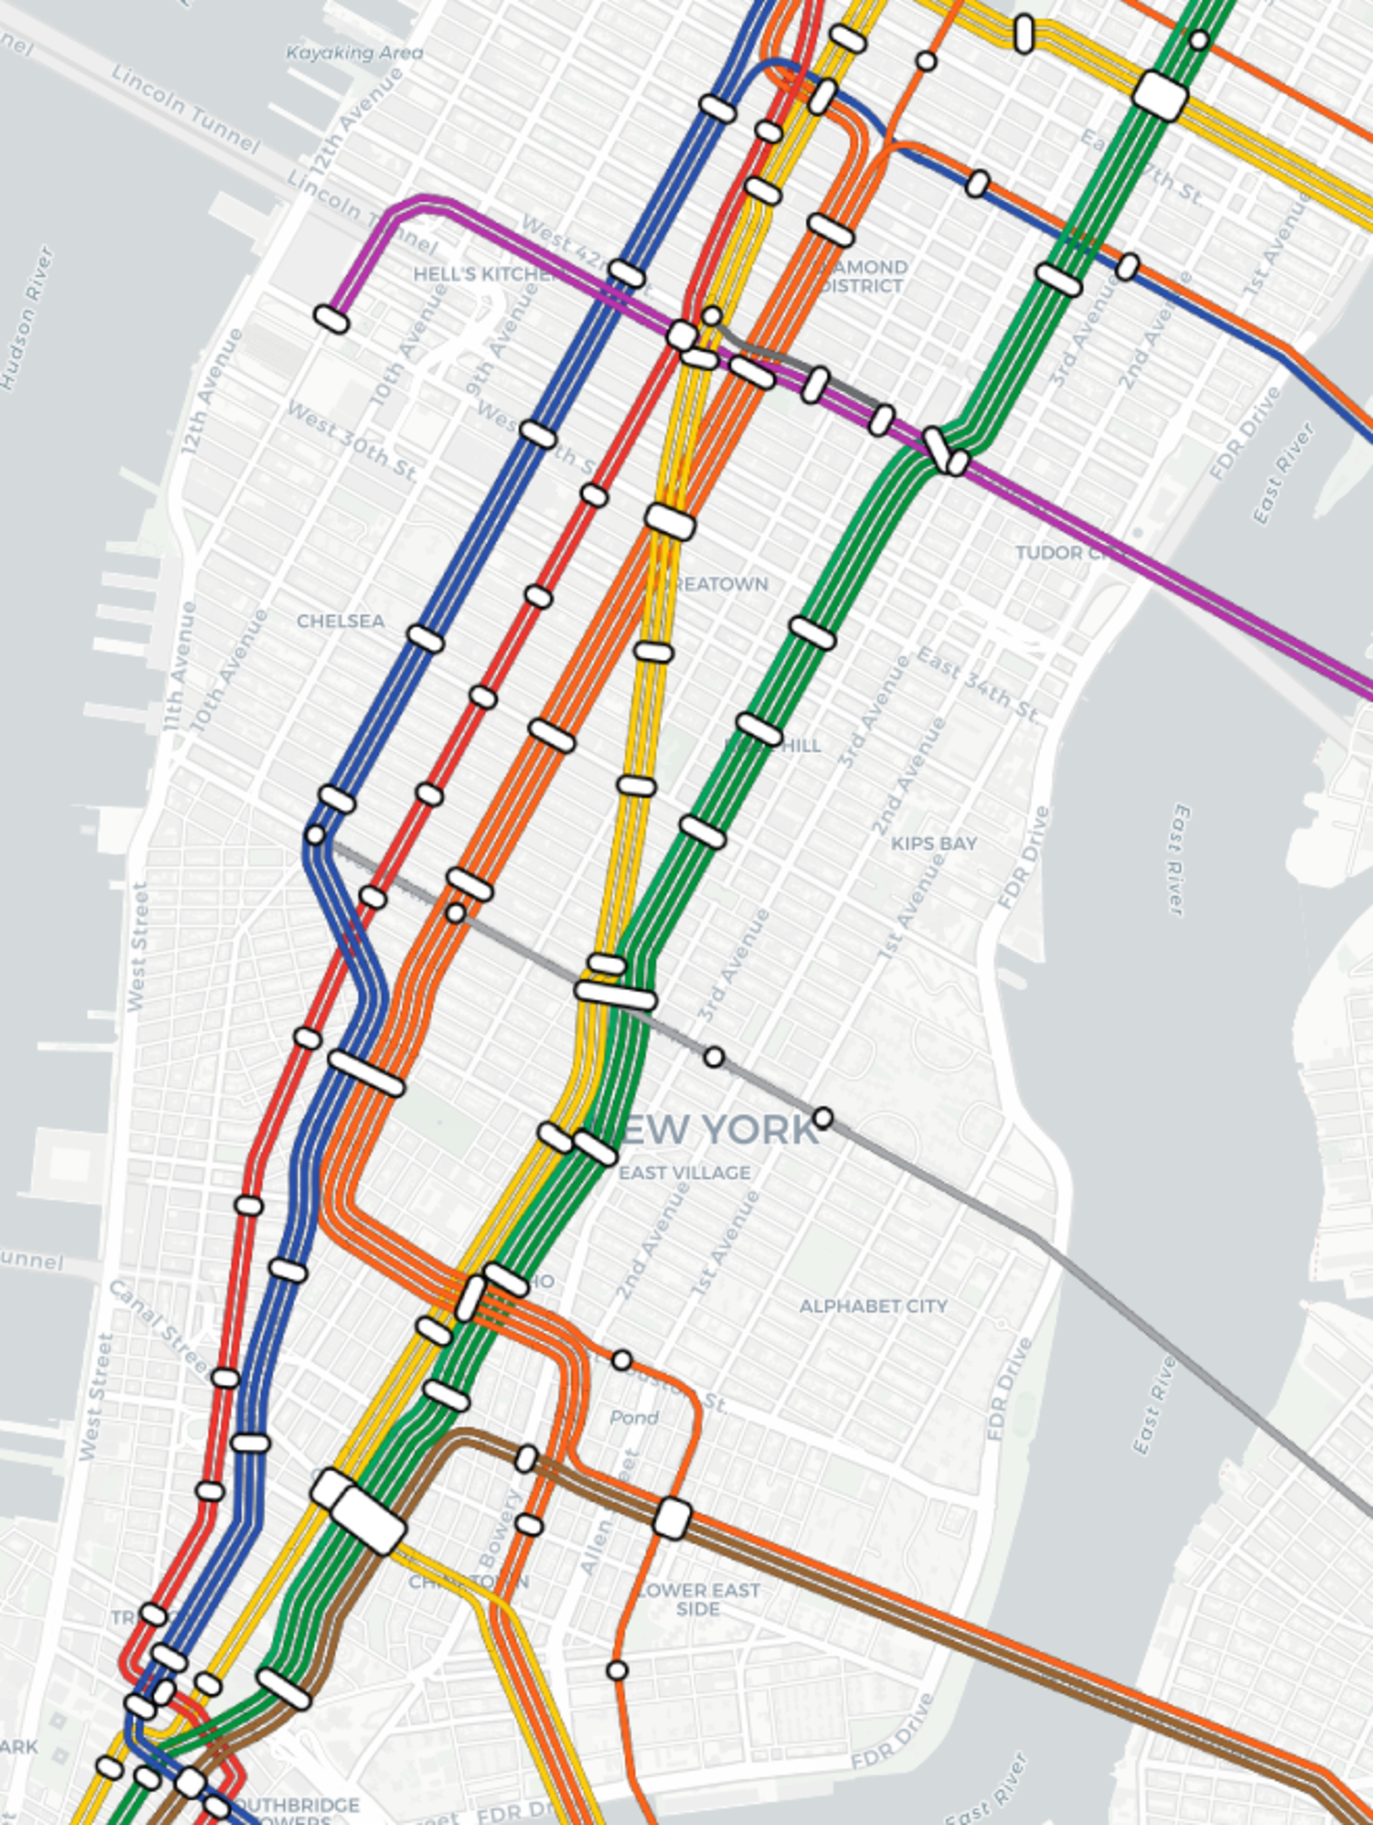
\includegraphics[width=0.47\textwidth]{newyork.pdf}
% \caption{Automatically generated map of the NYC subway. Express lines have been uncollapsed to artificially increase the line graph complexity.}
%\vspace{-1em}
% \end{figure}


\begin{figure*}[t]
  \centering
  \includestandalone[trim={19pt, 3pt, 0, 0}, clip, width=0.46\textwidth]{render_examples/vvs_transit_graph}
  \hspace{0.5cm}
  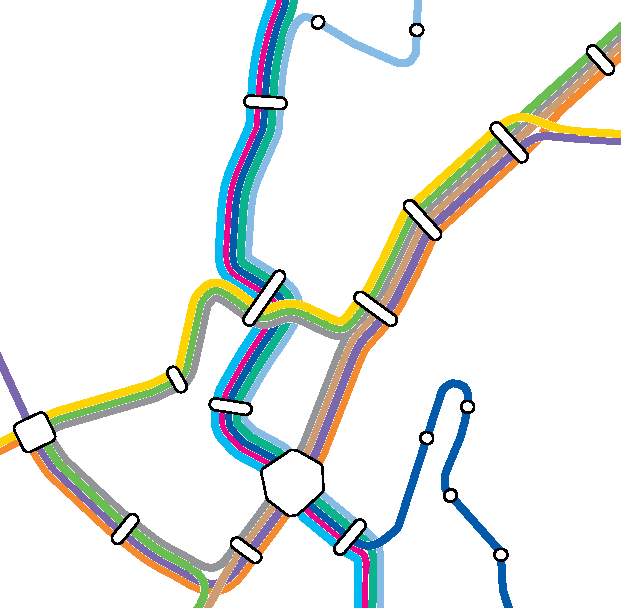
\includegraphics[trim={0cm 0 2.47cm 4.07cm},clip,width=0.46\textwidth]{render_examples/vvs_cropped.pdf}
  \caption{Left: Excerpt from a line graph which LOOM constructed from the GTFS data for the 2015 light rail network of the city of Stuttgart. Each edge corresponds to a segment of the network where the same set of lines takes the same geographical course. Segment boundaries are often station nodes (large) but may also be intermediate nodes (small). The line ids for each segment are given in ascending order. LOOM's central optimization step computes a line ordering for each segment. This determines how the lines are drawn in the map, and where line crossings and separations occur. Right: The corresponding excerpt from LOOM's transit map.}
  \label{FIG:transitgraphvvs}  
  %\vspace{-0.4cm}
\end{figure*}


\begin{enumerate}[parsep=0.5mm, wide, labelwidth=0mm, itemindent=2.3mm]
  \setlength\itemsep{0pt}
\item  It should depict the topology of the network: which transit lines are offered, which stations do they serve in which order, and which transfers are possible.
\item It should be neatly arranged and esthetically pleasing.
\item It should reflect the geographical course of the lines, at least to some extent.
\end{enumerate}

\smallskip\noindent
So far, such maps have been designed and drawn by hand.
Concerning (3), the designers usually take some liberty, either to make the map fit into a certain format or to simplify the layout, or both.

%\noindent
The goal of this paper is to produce transit maps fully automatically, adhering to (3) rather strictly: within a given tolerance, the lines on the map should be drawn according to their geographical course. This gives rise to several algorithmic challenges; in particular because the geographical course of some lines may overlap partially. These lines should then of course not be rendered on top of each other as this would obfuscate the visibility. Instead, they should be drawn next to each other. This requires to first identify overlapping parts and then to choose the line ordering in the rendered map. A bad ordering can lead to many unnecessary line crossings. Hence our goal is to find orderings that minimize these undesired crossings. As the number of possible orderings exceeds an octillion even for the transit network of medium sized cities, we need to develop efficient methods to find the best ordering in reasonable time.

\def\Hl{L}

\subsection{Overview and Definitions}\label{SEC:intro:definition}

LOOM proceeds in three stages, which we briefly describe in the following along with some notation and terminology that will be used throughout the paper.
(1) given the line data, construct the line graph; (2) compute an optimal line ordering for each edge via an ILP; (3) from the line graph and the line ordering, render the map.
Each stage is described in more detail in one of the following sections.

\smallskip\noindent
{\bf Input:}
The input to LOOM is a set ${\cal S}$ of stations and a set ${\cal L}$ of lines.
Each station has a geographical location.
Each line has a unique ID (in our examples: numbers), and information about the sequence of stations it serves, and the geographical course between them.
This data is usually provided as part of a network's GTFS feed.
% \footnote{If the information about the geographical course of the lines is missing, a good approximation is to compute shortest paths on the relevant underlying network.}

\smallskip\noindent
{\bf Line graph construction (Sect.~\ref{SEC:graph}):}
In its first stage, LOOM computes a \emph{line graph}.
This is an undirected labeled graph $G = (V, E, \Hl)$, where $V \supseteq {\cal S}$ (each station is a node, but there may be additional nodes), $E$ is the set of edges, and each $e \in E$ is labeled with a subset $\Hl(e) \subseteq {\cal L}$ of the lines.
Intuitively, each edge corresponds to a segment of the network, where the same set of lines takes the same geographical course (within a certain tolerance), and there is a node wherever such a set of lines splits up in different directions.
Fig.~\ref{FIG:transitgraphvvs}, left shows the line graph for an excerpt from the light rail network of Stuttgart.
We will see that the complexity of our algorithms in Sect.~\ref{SEC:ordering} depends on $M = \max_{e \in E} |\Hl(e)|$, the maximal number of lines per segment.
The line graph construction is described in Sect.~\ref{SEC:graph}.

\smallskip\noindent
{\bf Line ordering optimization (Sect.~\ref{SEC:ordering}):}
In its second stage, LOOM computes an \emph{ordering} of $\Hl(e)$ for each $e \in E$.
This ordering determines where line crossings and separations occur, and is hence critical for the final map appearance.
Previous research referred to the problem of minimizing crossings as the metro-line crossing minimization problem (MLCM), see Sect~\ref{SEC:related}. We formulate two strongly related problems: the metro-line node crossing minimization problem (MLNCM), and a variant with a line separation penalty (MLNCM-S). We formulate a concise Integer Linear Program (ILP) to solve instances of these problems.

\smallskip\noindent
{\bf Rendering (Sect.~\ref{SEC:rendering}):}
In its third stage, LOOM draws the transit map based on the line graph from stage 1 and the ordering from stage 2.
Each station node $v$ is drawn as a polygon, where each side of the polygon corresponds to exactly one incident edge of $v$.
We call this side the \emph{node front} of that edge at that node.
The node front for an edge $e$ has $|\Hl(e)|$ so-called \emph{ports} (Fig.~\ref{FIG:crossings}).
Drawing the map then amounts to connecting the ports (according to the ordering computed in stage 2) and drawing the station polygons.
Fig.~\ref{FIG:transitgraphvvs}, right shows a rendered transit map after layout optimization.

\subsection{Contributions}\label{SEC:intro:contrib}
\begin{itemize}[parsep=0.5mm,leftmargin=4mm]
\renewcommand\labelitemi{$\bullet$}
\item We present a new automatic map generator, called LOOM (Line-Ordering Optimized Maps), for geographically accurate transit maps. The input is basic schedule data as provided in a GTFS feed.
 This is, as far as we know, the first research paper on this problem in its entirety. Previous research work considers only parts of this problem (oblivious either to the geographical course or to the order of the lines) and does not yield maps that can be used for tiles and overlays in typical map services.

\item We describe a line-sweeping approach to extract the line graph from a set of (partially overlapping) vehicle trips as they occur in real-world schedule data.
\item We phrase the crossing minimization problem in a novel way and provide an ILP formulation to solve it. Our new model resolves some issues with previous models, in particular, the restricted applicability of some algorithms to planar graphs, and the necessity of artificial grouping of crossings (which happens naturally with our approach).

\item As a naive ILP formulation turns out to lead to impractically many constraints, we derive an alternative formulation yielding significantly smaller ILPs in theory and practice.

\item We describe engineering techniques which allow to further simplify the line graph and hence lead to even smaller ILPs without compromising optimality of the final result.

\item We evaluate LOOM on the transit network of six cities around the world.
For each city, line graph construction, ILP solution and rendering together take less than 15 seconds.

\item Our maps are publicly available online\footnote{\url{http://loom.informatik.uni-freiburg.de}}.
\end{itemize}

%%
%\subsection{Contribution}\label{SEC:contrib}
%%
%
%We describe an approach for automated drawing of transit maps that can be used with arbitrary schedule data as input. For medium sized urban rail networks, rendering usually only takes a few seconds. A crucial difference of previous approaches to our work is the strong abstraction from the geometry of the transit map. In prior publications, the graph used for optimization is constructed upon the stations which serve as nodes and the transit lines which induce edges between those nodes. But the original embedding of the edges is not taken into account, and crossings are allowed to occur anywhere along the edges (except their endpoints). As we aim for a truthful presentation of vehicle paths in our map, we do not ignore the shape of the lines between stations. Instead, we introduce a new graph model for transit maps where nodes represent topology changes in the embedding and edges represent parallel line segments. This allows us to restrict crossing events to nodes (without hiding them behind station markers!). Our approach resolves some issues with the MLCM model, as e.g. the restricted applicability of some algorithms to planar graphs, and the necessity of artificial grouping of crossings (which happens naturally with our approach).
%
%We describe a line-sweeping approach to extract this graph from a set of (partially overlapping) vehicle trips as they occur in real-world schedule data. To solve the line-crossing problem in our model, we first build a baseline ILP and then develop an improved version of this program. We introduce a line-partner separation penalty and describe an extension to the ILP that optimizes the number of separations. To further simplify the problem, we give some explicit rules to reduce the graph to an optimality-preserving core problem graph.
%
%We also briefly discuss some heuristics for the placement of inevitable crossings and describe how a map can be rendered from our model. Our method is evaluated be running it against several real-world public transit schedules. The maps have been published online\footnote{\url{http://panarea.informatik.uni-freiburg.de/gtfs-lines}}.
%

%
\subsection{Related Work}\label{SEC:related}
%
\subsubsection{Map Construction and Edge Bundling}

The first step in our pipeline -- the line graph construction -- is closely related to map construction and edge bundling. 

The goal of  \emph{map construction} algorithms is producing the graph of an underlying (street) network from vehicle trajectory data. There is a variety of map construction algorithms described in the literature; see \cite{ahm15} for an overview. For example, in \cite{ahm12}, an incremental approach is used which starts with an empty map and incrementally updates the network graph with new trajectories. New trajectories are partially map-matched to existing graph segments with a global distance threshold and their geometries updated accordingly, while unmatched parts introduce new edges (and thus intersection nodes). The main difference between existing work (on street networks) and our approach is that our input data already represents a multigraph (with stations as intersection nodes) and is usually quite sparse. 
%Regarding an exact reconstruction of the network, we accept a loss of accuracy as a (desired) map simplification. This makes the problem  easier to handle; and we found that incrementally collapsing segment parts that are within a (perpendicular) threshold distance already yields good results.

The goal of \emph{edge bundling} in general networks is to group edges in order to save ink when drawing the network. Usually, the embedding of the edges is not fixed a priori but can be chosen such that many bundles occur (possibly respecting side constraints, like edges being short). For example, in \cite{hol09} a force-directed heuristic was described where edges attract other edges to form bundles automatically. For our problem, we are not allowed to embed edges arbitrarily as we want to maintain the geographical course of the vehicle trajectories. In \cite{pup11}, edge bundling in the context of metro line map layout was discussed, also considering orderings within the bundles to minimize crossings. But for their approach to work, the underlying graph has to fulfill a set of restrictive properties. For example, the so called \emph{path terminal property} demands that a node in the graph cannot be an endpoint of one line and an intermediate node of another line at the same time. But this structure regularly appears in real-world datasets. For example, a local train might end at the main station of a town, while a long-distance train might have this station only as an intermediate stop. Also self-intersections are forbidden which excludes instances with cyclic subway lines. With these additional properties required in \cite{pup11}, the problem becomes significantly easier but is no longer compatible with most real-world datasets. In contrast, our line graph construction and subsequent crossing minimization algorithms are compatible with real-world inputs of arbitrary structure.

\subsubsection{Crossing Minimization}


Previous research on the metro-line crossing minimization problem (MLCM), as briefly summarized in the following, typically comes without experimental evaluations and without the production of actual maps.
The problem of minimizing intra-edge crossings in transit maps was introduced in~\cite{ben06},
with the premises of not hiding crossings under station markers for aesthetic reasons.
A polynomial time algorithm for the special case of optimizing the layout along a single edge was described.
The term MLCM was coined in~\cite{bek07}.
In that paper, optimal layouts for path and tree networks were investigated but arbitrary graphs were left as an open problem.
In~\cite{arg08, arg10, nol09}, several variants of MLCM were defined and efficient algorithms were presented for some of these variants, often with a restriction to planar graphs.
In \cite{asq08}, an ILP formulation for MLCM under the periphery condition (lines ending in a station must be drawn at the left- or rightmost position in  incident edges, see Sect.~\ref{SEC:separation}) was introduced.
The resulting ILP was shown to have a size of $\mathcal{O}(|L|^2|E|)$ with $L$ being the set of lines and $E$ the set of edges in the derived graph.
In~\cite{fin13b}, it was observed that crossings scattered along a single edge are also not visually pleasing,
and hence crossings were grouped into so-called block crossings.
The problem of minimizing the number of block crossings was shown to be NP-hard on simple graphs just like the original MLCM problem \cite{fin13a}.
Our adapted MLNCM problem has the same complexity as MLCM and is hence also NP-hard.


\subsubsection{Schematic Metro Maps}

Another line of research focuses on drawing \emph{schematic} metro maps, for example, by restricting the representation of transit lines to octilinear polylines~\cite{hon06} or B\'ezier Curves~\cite{fin12}. See \cite{nol14} for a recent survey on automated metro map layout methods. These approaches strongly abstract from the geographical course of the lines (and often also from station positions), and the minimization of line crossings or separations is not part of the problem.
In particular, the resulting maps cannot be used for tiles or overlays in typical map services.

There is also some applied work on transit maps, but without publications of the details.
One approach that seems to use a model similar to ours was described by Anton Dubreau in a blog post~\cite{dub16} although without a detailed discussion of their method. As far as we are aware there are no papers on MLCM that deal with real public transit data.

%
\section{Line Graph Construction}\label{SEC:graph}
%
\begin{figure}[t]
  \centering
  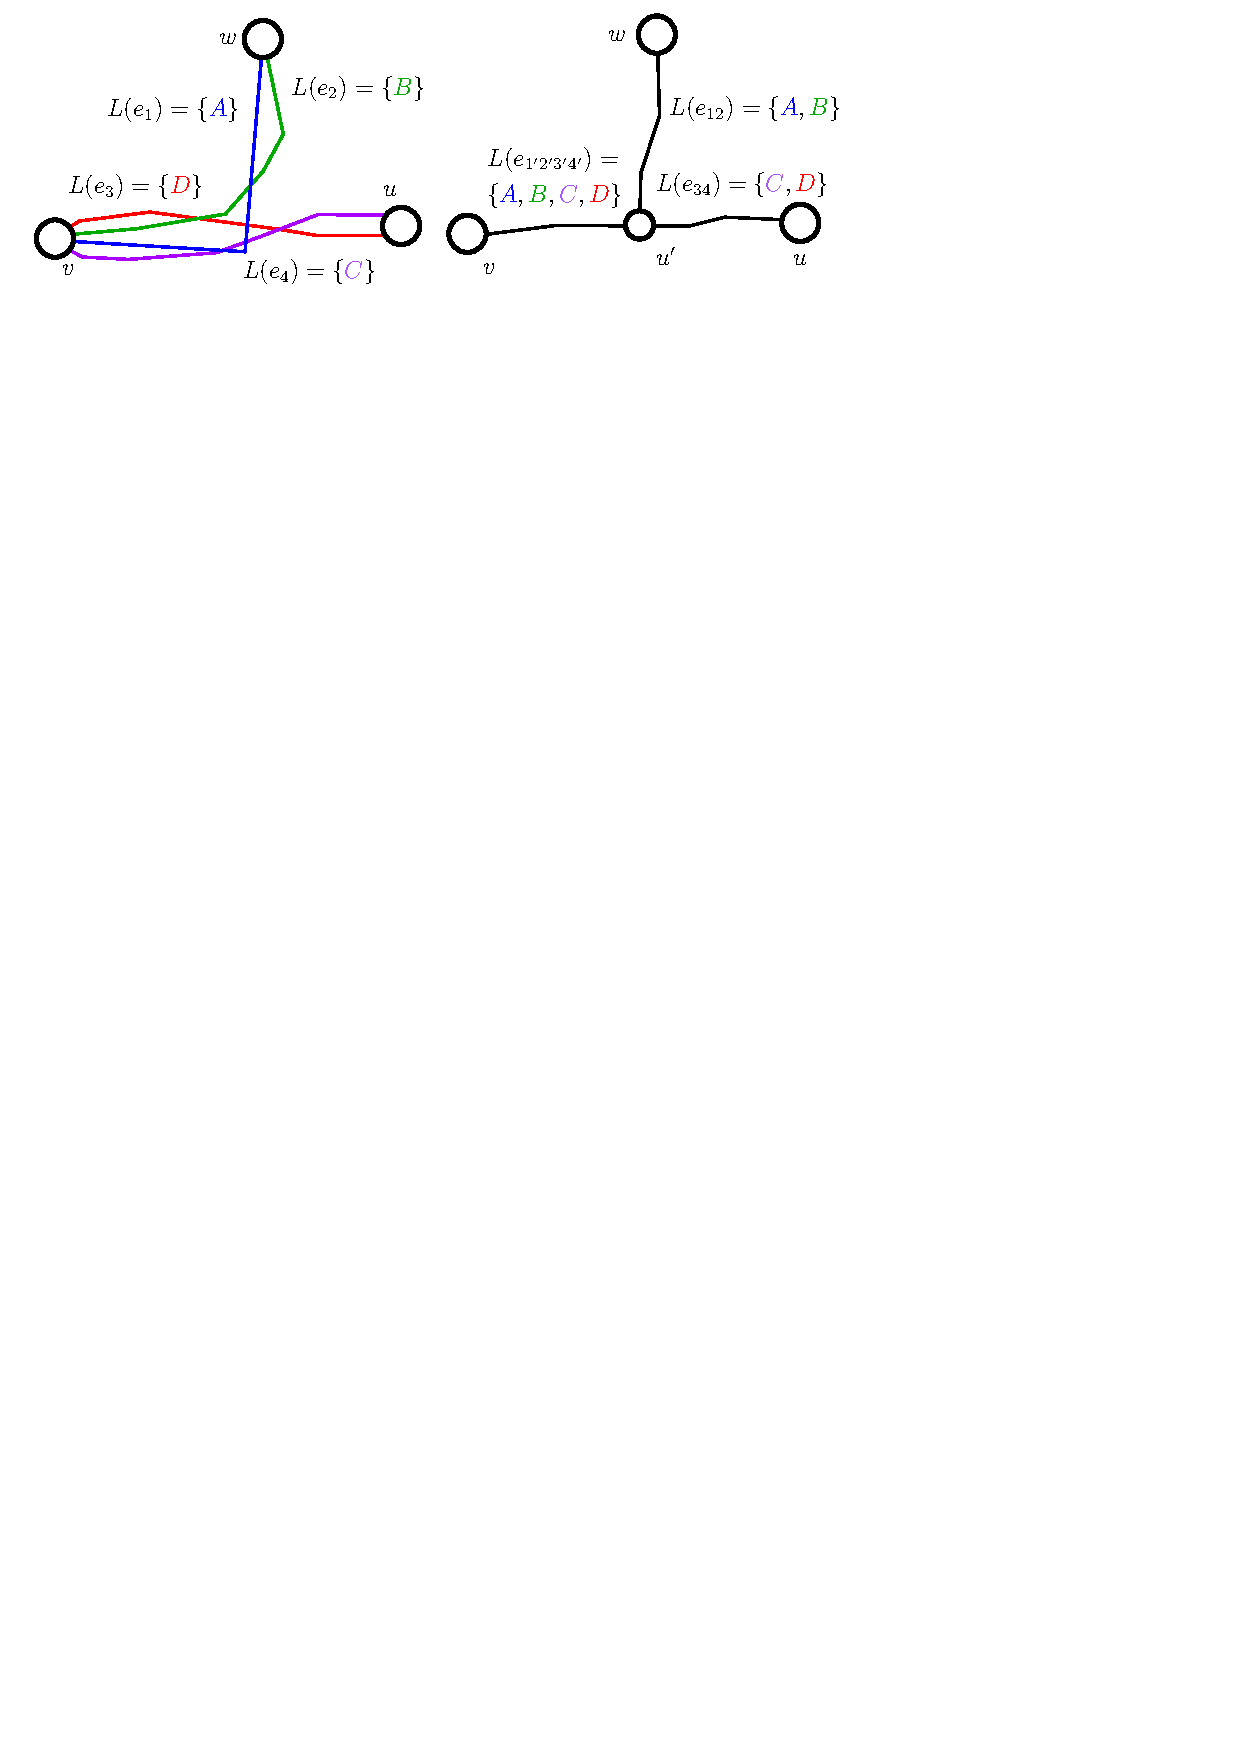
\includegraphics[width=0.7\textwidth]{linegraph.pdf}
  \caption{Left: Input multigraph $G^0$ created from schedule data (GTFS). Nodes represent stations, and each edge holds a single line that occurs between two stations. There may be many overlapping edge segments. Right: Line graph $G$ constructed from $G^0$ by repeatedly combining shared edge segments into a single, new edge. The overlapping segments have been collapsed, and a new node $u'$ was introduced at the segment boundaries.}  
  \label{FIG:linegraph}
  %\vspace{-0.4cm}
\end{figure}

This section describes stage 1 of LOOM: given line data, construct the line graph.
We assume that the data is given in the GTFS format \cite{gtfs}.
In GTFS, each trip (that is, a concrete tour of a vehicle of a line) is given explicitly and the graph $G^0$ formed by all station coordinates and the trips between them has many overlapping edges that may (partially) share the same path (Fig.~\ref{FIG:linegraph}, left).

Let $e_1, e_2$ be two edges in $G^0$ with geometrical paths $\tau_1$ and $\tau_2$. For each $\tau$, we define a parametrization $p_\tau(t): [0,1] \mapsto \mathbb{R}^2$ which maps the progress $t$ to a point on $\tau$ (e.g., if the length of $\tau$ is 10 meters, $p_\tau(\frac{1}{2})$ returns the point we would reach after travelling on $\tau$ for $5$ meters). We call $(t, t'), t' \geq t$ a segment of $e$. To decide whether a segment $(t_1, {t_1}')$ of $e_1$ is similar to a segment $(t_2, {t_2}')$ of $e_2$, we use a simple approximation. For a distance threshold $\hat{d}(e_1, e_2)$, we say $\left(\left(t_1, t_2\right), \left({t_1}', {t_2}'\right)\right)$ is a shared segment of $e_1$ and $e_2$ if
\begin{equation}
	\forall u \in [t_1, {t_1}']: \exists u' \in [t_2, {t_2}']:\left\|p_{\tau_1}(u) - p_{\tau_2}(u')\right\| \leq \hat{d}(e_1, e_2),
\end{equation}
that is, if for every point $p_{\tau_1}(u)$ on $\tau_1$, there exists a corresponding point $p_{\tau_2}(u')$ on $\tau_2$ within the threshold distance $\hat{d}(e_1, e_2)$.

As we want to avoid overlapping lines during rendering, we have to chose $\hat{d}(e_1, e_2)$ in such a way that there will be enough space between the edges in the final line graph. Let $w$ be the desired width of a single line in the rendered map. The definition
\begin{equation}
\hat{d}(e_1, e_2) = \frac{w|L(e_1)| + w|L(e_2)|}{2}
\end{equation}
satisfies this, as we need $w|L(e)| / 2$ map units of space on either side of $e$ to render all $l \in L(e)$ with width $w$ (see Sect.~\ref{SEC:rendering}).

We transform $G^0$ into a line graph $G$ by repeatedly combining a shared segment between two edges $e_1 = \{u_1, v_1\}$ and $e_2 = \{u_2, v_2\}$ into a single new edge $e_{12}$ until no more shared segments can be found. The path $\tau_{12}$ of $e_{12}$ is averaged from the shared segments on $e_1$ and $e_2$, and we set $L(e_{12}) = L(e_1) \cup L(e_2)$ (Fig.~\ref{FIG:linegraph}, right). Two new non-station nodes $u'$ and $v'$ which mark the beginning and end of the shared segment are introduced and split $e_1$ and $e_2$ such that $e_1 = \{u_1, u'\}$, $e_2 = \{u_2, u'\}$, $e'_1 = \{v', v_1\}$, $e'_2 = \{v', v_2\}$ and $e_{12} = \{u', v'\}$. Note that the new non-station nodes $v'$ and $u'$ will always have a degree of 3. After each iteration, we obtain from $G^i$ a new graph $G^{i+1}$. If the distance between a node $v'$ added to $G^{i+1}$ and an existing node $v$ in $G^i$ is smaller than $\hat{d}(e_1, e_2)$ after collapsing an $e_1$ and $e_2$, we merge $v$ and $v'$ to avoid cluttering the graph with many start and end nodes of shared segments. 

To find the shared segments between $e_1$ and $e_2$, we sweep over $\tau_1$ in $n$ steps of some $\Delta t$, measuring the distance $d$ between $p_{\tau_1}(i\cdot\Delta t)$ and $\tau_2$ at each $i < n$ along the way. If $d \leq \hat{d}(e_1, e_2)$, we start a new shared segment. If $d > \hat{d}(e_1, e_2)$ and a shared segment is open, we close it. For our test datasets, we found that a $\Delta t$ of 10 meters is usually small enough to achieve satisfying results.

The algorithm can be made more robust against outliers by allowing $d$ to exceed $\hat{d}(e_1, e_2)$ for a number of $k$ steps. It can be sped up by indexing every linear segment of every path in a geometric index. Just like in previous work on incremental map construction, the results of our algorithm depend on the order in which the segments are combined. For our evaluation in Sect.~\ref{SEC:eval}, we used a random order.

%
\section{Line Ordering Optimization}\label{SEC:ordering}
%

This section describes stage 2 of LOOM, namely how to solve MLNCM: given a line graph, compute an ordering of the lines for each edge such that the total number of  crossings in the final map is minimized. Contrary to the classic MLCM problem, which imposes a right and left ordering on each $L(e)$ and allows crossings to occur anywhere on $e$, MLNCM only imposes a single ordering on each edge and restricts crossing events to nodes. This will prove advantageous during rendering, see Sect.~\ref{SEC:rendering}. As the set of stations $\cal S$ is only a subset of $V$ in our model (Sect.~\ref{SEC:intro:definition}), we can still avoid line crossings in them.

%
\def\Hsum{\sum\nolimits}
\subsection{Baseline ILP}\label{SEC:baseline}
\begin{figure}
  \centering
  $\vcenter{\hbox{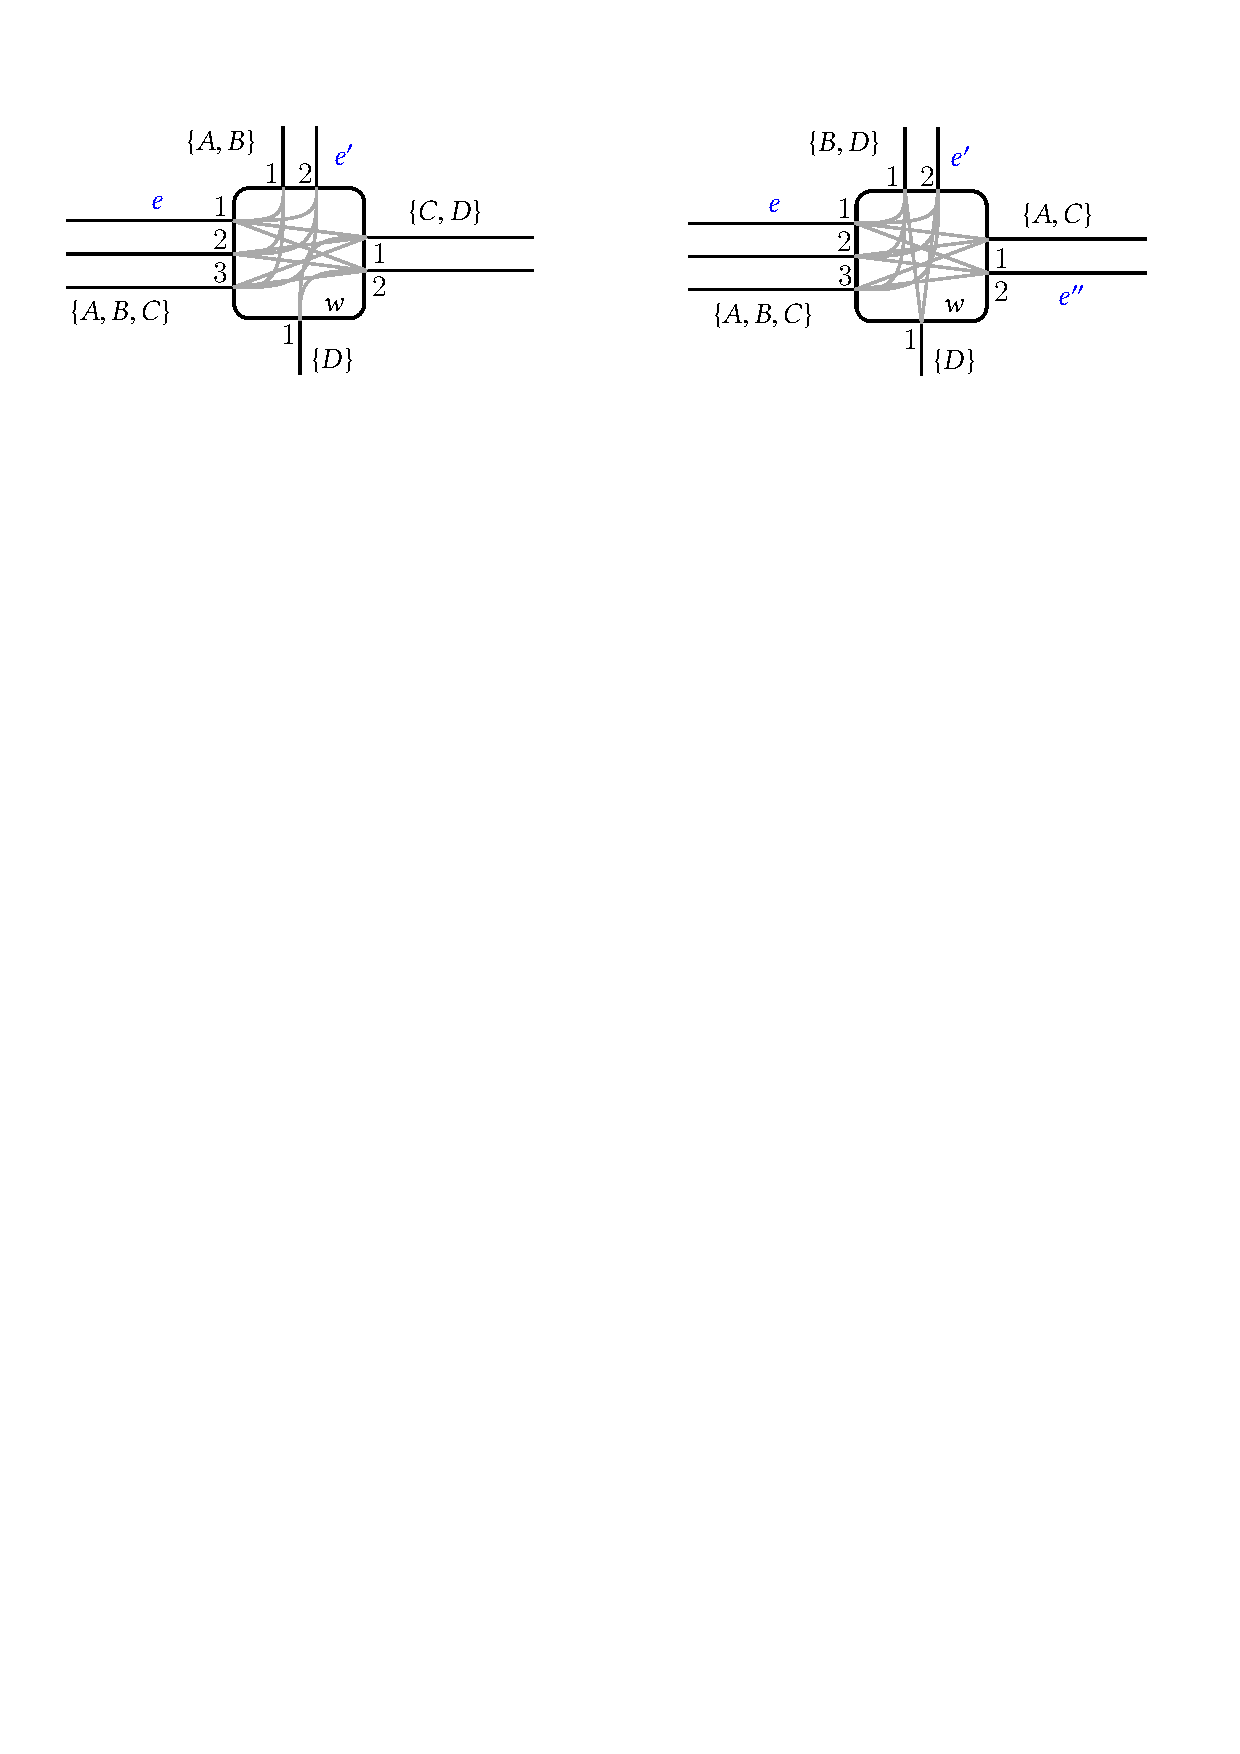
\includegraphics[width=0.67\textwidth]{crossing.pdf}}}$
  \caption{Example instances. Both station polygons have 4 \emph{node fronts}, each corresponding to an incident edge. Each node front has exactly one port ($1, 2, ...$) for each line traversing through its edge. Gray lines depict possible inner node connections. Left: $A, B$ extend from $e$ to $e'$ over $w$ and may introduce a crossing, if the position of $A$ is smaller than the position of $B$ in $e$, but not in $e'$ (or vice versa). Right: a crossing between $A$ and $B$ only depends on the line ordering in $e$, but not on the orderings in $e'$ and $e''$.}
  \label{FIG:crossings}
\end{figure}
%
For each edge $e$, there are $|\Hl(e)|!$ many orderings, therefore the total number of combinations for the whole graph is immense.
We formulate an ILP to find an optimal solution.
We first define a baseline ILP which explicitly considers line crossings and has $\mathcal{O}(|E|M^{2})$ variables and $\mathcal{O}(|E|M^{6})$ constraints.
We then define an improved ILP with only $\mathcal{O}(|E|M^2)$ constraints and which also considers line separations (MLNCM-S).

For every edge $e \in E$, we define $\left|L\left(e\right)\right|^{2}$ decision variables $x_{elp} \in \{0,1\}$ where $e$ indicates the edge, $l \in L(e)$ indicates the line, and $p=1, ..., \left|L\left(e\right)\right|$ indicates the position of the line in the edge. We want to enforce $x_{elp}=1$ when line $l$ is assigned to position $p$, and $0$ otherwise. This can be realized with the following constraints:
\begin{equation}
\forall l \in L(e): \Hsum_{p=1}^{|L(e)|} x_{elp}=1.  \label{EQ:p_constr1_bl}
\end{equation}
%
To ensure that exactly one line is assigned to each position, we need the following additional constraints:
%
\begin{equation}
	\forall p \in  \left\{1,...,\left|L\left(e\right)\right|\right\} : \Hsum_{l \in L(e)} x_{elp} = 1. \label{EQ:p_constr2_bl}
\end{equation}%\subsubsection{Avoiding crossings}\label{SEC:ac}
Let $A, B$ be two lines belonging to an edge $e = \{v,w\}$ and both extend over $w$.
We distinguish two cases: either $A$ and $B$ continue along the same adjacent edge $e'$ (Fig.~\ref{FIG:crossings}, left), or they continue along different edges $e'$ and $e''$ (Fig.~\ref{FIG:crossings}, right).

In the first case, $A$ and $B$ induce a crossing if the position of $A$ is smaller than the position of $B$ in $L(e)$, so $p_e(A) < p_e(B)$, but vice versa in $L(e')$. We introduce the decision variable $x_{ee'AB} \in \{0,1\}$, which should be $1$ in case a crossing is induced and $0$ otherwise. To enforce this, we create one constraint per possible crossing. For example, a crossing would occur if we have $p_e(A)=1$ and $p_e(B)=2$ as well as $p_{e'}(A)=2$ and $p_{e'}(B) =1$. We encode this as follows:
\begin{align}
	x_{eA1} + x_{eB2} + x_{e'A2} + x_{e'B1} - x_{ee'AB} \leq 3  \label{EQ:crossdec_constr_bl}.
\end{align}
In case the crossing occurs, the first four variables are all set to 1. Hence their sum is 4 and the only way to fulfill the $\leq 3$ constraint is to set $x_{ee'AB}$ to $1$. In the example given in Fig.~\ref{FIG:crossings}, six such constraints are necessary to account for all possible crossings of the lines $A$ and $B$ at node $w$.
The objective function of the ILP then minimizes the sum over all variables $x_{ee'AB}$.

In the second case, the actual positions of $A$ and $B$ in $e'$ and $e''$ do not matter, but just the order of $e'$ and $e''$. We introduce a split crossing decision variable $x_{ee'e''AB} \in \{0,1\}$ and constraints of the form $x_{eAi} + x_{eBj} - x_{ee'e''AB} \leq 1$ for all orders of $A$ and $B$ at $e$ with $i < j$ as in that case a crossing would occur.
We add $x_{ee'e''AB}$ to the objective function.

\subsubsection{ILP size}
For mapping lines to positions at each edge we need at most $|E|M^{2}$ variables and $2|E|M$ constraints. To minimize crossings, we have to consider at most $M^{2}$ pairs of lines per edge, and introduce a decision variable for each such pair. That makes at most $|E| M^{2}$ additional variables, which all appear in the objective function. Most constraints are introduced when two lines continue over a node in the same direction. In that case, we create no more than $\binom{M}{2}^{2} < M^{4}$ constraints per line pair per edge, so at most $|E| M^{6}$ in total.
In summary, we have $\mathcal{O}(|E|M^{2})$ variables and $\mathcal{O}(|E|M^{6})$ constraints.

\begin{figure*}[t]
\centering
\begin{minipage}{.48\textwidth}
  \centering
  %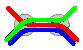
\includegraphics[trim={2.25 0 2.25 0},clip,angle=270,origin=c,width=.25\textwidth]{render_examples/splitting_example_nonopt.pdf}\hspace{19pt}
  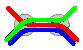
\includegraphics[trim={2.25 2.2 2.25 2.2},clip,width=.45\textwidth]{render_examples/splitting_example_nonopt.pdf}\hfill
  %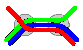
\includegraphics[trim={2.25 0 2.25 0},clip,angle=270,origin=c,width=.25\textwidth]{render_examples/splitting_example.pdf}
  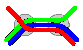
\includegraphics[trim={2.25 2.2 2.25 2.2},clip,width=.45\textwidth]{render_examples/splitting_example.pdf}
  %\caption{Crossings are minimized in the left example (1), but the right example with 2 crossings better indicates line pairings.}
  \caption{Minimized crossings in the left example, but the right example better indicates line pairings.}
  \label{FIG:linesplitting}
\end{minipage}%
\hfill
\begin{minipage}{.48\textwidth}
  \centering
  %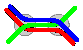
\includegraphics[trim={2.25 0 2.25 0},clip,angle=90,origin=c,width=.25\textwidth]{render_examples/splitting_example2_nonopt.pdf}\hspace{19pt}
  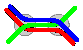
\includegraphics[trim={2.25 2.2 2.25 2.2},clip,width=.45\textwidth]{render_examples/splitting_example2_nonopt.pdf}\hfill
  %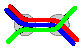
\includegraphics[trim={2.25 0 2.25 0},clip,angle=90,origin=c,width=.25\textwidth]{render_examples/splitting_example2.pdf}
  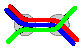
\includegraphics[trim={2.25 2.2 2.25 2.2},clip,width=.45\textwidth]{render_examples/splitting_example2.pdf}
  \caption{Both orderings have 2 crossings, but in the right example they are done in one pass.}
  \label{FIG:linesplitting2}
\end{minipage}
\end{figure*}

%
\subsection{Improved ILP Formulation}\label{SEC:improved}
%
The $\mathcal{O}(|E|M^{2})$ variables in the baseline ILP seem to be reasonable, as indeed $\Omega(|E|M^{2})$ crossings could occur. But the $\mathcal{O}(|E|M^{6})$ constraints are due to enumerating all possible position inversions explicitly. If we could check the statement \emph{position of A on $e$ is smaller than the position of B} efficiently, the number of constraints could be reduced. To have such an oracle, we first modify the line-position assignment constraints.

\subsubsection{Alternative line-position assignment}
Instead of a decision variable encoding the exact position of a line, we now use $x_{el\leq p} \in \{0,1\}$ which is $1$ if the position of $l$ in $e$ is $\leq p$ and $0$ otherwise. To enforce a unique position, we use the constraints:
\begin{align}
	\forall l \in L(e)~ \forall p \in \{1, ..., \left|L\left(e\right)\right|-1\}: \quad x_{el\leq p} \leq x_{el\leq p+1}. \label{EQ:up_constr}
\end{align}
This ensures that the sequence can only switch from $0$ to $1$, exactly once. To make sure that at some point a $1$ appears and that each position is occupied by exactly one line, we additionally introduce the following constraints:
\begin{align}
	\forall p \in \{1, ..., \left|L\left(e\right)\right|\}: \quad  \Hsum_{l \in L(e)} x_{el\leq p} = p. \label{EQ:01_constr}
\end{align}
So for exactly one line $l$, $x_{el\leq 1} = 1$, for exactly two lines $l'$ and $l''$, $x_{el'\leq 2} = x_{el''\leq 2} = 1$ (where for one $l \in \{l',l''\}$, $x_{el\leq 1} =1$) and so on.

\subsubsection{Crossing Oracle}
We reconsider the example in Fig.~\ref{FIG:crossings}, left. Before, we enumerated all possible positions which induce a crossing for $A, B$ at the transition from $e$ to $e'$. But it would be sufficient to have variables which tell us whether the position of $A$ is smaller than the position of $B$ in $e$, and the same for $e'$, and then compare those variables. For a line pair $(A,B)$ on edge $e$ we call the respective variables $x_{eB<A}, x_{eA<B} \in \{0, 1\}$. %Since we introduce these variables for each line pair in $e$, $x_{eA<B}$ will re-appear as $x_{eB>A}$, so we only need $x_{eA>B}$.
To get the desired value assignments, we add the following constraints:
\begin{gather}
	\Hsum_{p=1}^{\left|L\left(e\right)\right|} x_{eA\leq p} - \Hsum_{p} x_{eB\leq p} + x_{eB<A} M \geq 0 \\
	x_{eB<A} + x_{eA<B}=1.
\end{gather}
The equality constraints make sure that not both $x_{eA<B}$ and $x_{eB<A}$ can be $1$. If the position of $A$ is smaller than the position of $B$, then more of the variables corresponding to $A$ are $1$, and hence the sum for $A$ is higher. So if we subtract the sum for $B$ from the sum for $A$ and the result is $\geq 0$, we know the position of $A$ is smaller and $x_{eB<A}$ can be $0$. Otherwise, the difference is negative, and we need to set $x_{eB<A}$ to $1$ to fulfill the inequality. It is then indeed fulfilled for sure as the position gap can never exceed the number of lines per edge.

To decide if there is a crossing, we would again like to have a decision variable $x_{ee'AB} \in \{0,1\}$ which is $1$ in case of a crossing and $0$ otherwise. The constraint
\begin{gather}
	\left|x_{eA<B}-x_{e'A<B}\right| - x_{ee'AB} \leq 0
\end{gather}
realizes this, as either $x_{eA<B} = x_{e'A<B}$ (both $0$ or both $1$) and then $x_{ee'AB}$ can be $0$, or they are not equal and hence the absolute value of their difference is $1$, enforcing $x_{ee'AB}=1$. As absolute value computation cannot be part of an ILP we use the following equivalent standard replacement:
\begin{align}
	x_{eA<B} - x_{e'A<B} - x_{ee'AB} &\leq 0 \label{EQ:abs_upper}\\
	-x_{eA<B} + x_{e'A<B} - x_{ee'AB} &\leq 0. \label{EQ:abs_lower}
\end{align}
If the values are equal, nothing changes in the argumentation. If the values are unequal, either (\ref{EQ:abs_upper}) or (\ref{EQ:abs_lower})  will produce a $1$ as the sum of the first two terms, enforcing $x_{ee'AB}=1$ as desired.

\subsubsection{Complexity of the improved ILP}

For the line-position assignment, we need at most $|E|M^{2}$ variables and constraints just like before.
For counting the  crossings, we need a constant number of new variables and constraints per pair of lines per edge.
Hence the total number of variables and constraints in the improved ILP is $\mathcal{O}(|E|M^{2})$.

\subsection{Preventing Line Partner Separation}\label{SEC:separation}

So far, we have only considered the number of crossings.
Another relevant criterion for esthetic appeal is that ``partnering'' lines are drawn side by side.
Fig.~\ref{FIG:linesplitting} and Fig.~\ref{FIG:linesplitting2} provide two examples. We address this by punishing line separations and call this extension to our original MLNCM problem \mbox{MLNCM-S}. For two adjacent edges $e$ and $e'$ and a line pair $(A, B)$ that continues from $e$ to $e'$, if $A$ and $B$ are placed alongside in $e$ but not in $e'$, we want to add a penalty to the objective function. For this, we add a variable $x_{eA\|B} \in \{0, 1\}$ which should be $0$ if $\left|p_{e}(A) - p_{e}(B)\right| = 1$ (if they are partners in $e$) and $1$ otherwise. As $x_{eA\|B} = x_{eB\|A}$, we define a set $U(e)$ of unique line pairs such that $(l, l') \in U(e) \Rightarrow (l', l) \not\in U(e)$. We add the following constraints per line pair $(A, B)$ in $U(e)$:
\begin{align}
	\Hsum_{p=1}^{\left|L\left(e\right)\right|} x_{eA\leq p} - \Hsum_{p} x_{eB\leq p} - x_{eA\|B} M &\leq 1 \label{EQ:sep_cstr_1} \\
	\Hsum_{p=1}^{\left|L\left(e\right)\right|} x_{eB\leq p} - \Hsum_{p} x_{eA\leq p} - x_{eA\|B} M &\leq 1. \label{EQ:sep_cstr_2}
\end{align}
If $|p_{e}(A) - p_{e}(B)| = 1$, then the sum difference is $\leq 1$ and $x_{eA\|B}$ can be 0. If $|p_{e}(A) - p_{e}(B)| > 1$, then either (\ref{EQ:sep_cstr_1}) or (\ref{EQ:sep_cstr_2}) enforce $x_{eA\|B} = 1$. To prevent the trivial solution where $x_{eA\|B}$ is always 1, we add the following constraint per edge $e$:
\begin{align}
	\Hsum_{(l, l') \in U(e)} x_{el\|l'} \leq \binom{\left|L\left(e\right)\right|}{2} - \left|L\left(e\right)\right| - 1,  \label{EQ:sep_cstr_3}
\end{align}
as there are $\binom{\left|L\left(e\right)\right|}{2}$ line pairs $(l, l') \in U(e)$ of which $\left|L\left(e\right)\right| - 1$ are next to each other.

Like in Sect.~\ref{SEC:improved}, we add a decision variable $x_{ee'A\|B}$ to the objective function that should be $1$ if $A$ and $B$ are separated between $e$ and $e'$ and $0$ otherwise:
\begin{align}
	x_{eA\|B} - x_{e'A\|B} - x_{ee'A\|B} &\leq 0 \\
	-x_{eA\|B} + x_{e'A\|B} - x_{ee'A\|B} &\leq 0.
\end{align}
%If $\left|L\left(e\right)\right| = |L(e')| = 2$, a line separation penalty is not needed for $A$ and $B$ because they will always be next to each other. If only $\left|L\left(e\right)\right| = 2$, we can add $x_{e'A\|B}$ to the objective function directly (and likewise if only $|L(e')|=2$).

As we only add 1 constraint per edge and a constant number of constraints and variables per line pair in each edge, the total number of variables and constraints remains $\mathcal{O}(|E|M^2)$.

\begin{figure}[b]
\centering
\begin{minipage}{.68\textwidth}
  \centering
  
\includegraphics[trim={0 0.9 0 1.8},clip,width=.49\textwidth]{render_examples/periphery/periphery_example1.pdf}
  \hfill
  
\includegraphics[width=.48\textwidth]{render_examples/periphery/periphery_example2.pdf}
  \caption{Left: Periphery condition guaranteed by separation penalty. Right: Periphery condition not guaranteed by separation penalty.}
  \label{FIG:periphery}
\end{minipage}
%\vspace{-.4em}
\end{figure}

\begin{figure*}[t]
\centering
  \includestandalone[width=6.1cm]{tikz/transitgraph_optim}
  \hfill
  \includestandalone[width=5.5cm]{tikz/coreoptimgraph}
  \hfill
  \includestandalone[width=6cm]{tikz/connected_components}
  \caption{Left: line graph $G$ with 7 lines. Middle: core graph of $G$ after applying pruning rules, $\{A, B\}$ was collapsed into $\{X\}$. Right: ordering-relevant connected components of $G$ after applying cutting rules.}
  \label{FIG:coreoptimgraph}
\end{figure*}

\subsubsection{Periphery Condition}
Interestingly, punishing line separations also addresses a special case of the periphery condition introduced in \cite{asq08}. In general, this condition holds if lines ending in a station are always drawn at the left- or rightmost position in each incident edge. For nodes with degree $\leq 2$, the periphery condition is trivially ensured in \mbox{MLNCM-S} (Fig.~\ref{FIG:periphery}, left). For other nodes, however, it is not guaranteed (Fig.~\ref{FIG:periphery}, right).

\subsection{Placement of Crossings or Separations}\label{SEC:crossing_placement}
The placement of crossings or separations may be fine-tuned by adding node-based weighting factors $w_\times(v)$ (for crossings) and $w_\|(v)$ (for separations) to the objective function to prefer nodes or to break ties. For example, $w_\times(v)$ may depend on the node degree.

As described above, we especially want to prevent crossings or separations in station nodes. This can be achieved by adding constant global weighting factors $w_{\cal S\times}$ and $w_{\cal S\|}$ to each $x_{ee'll'}$ and $x_{ee'l\|l'}$ in the objective function if $l$ and $l'$ continue over a node $v_s \in \cal S$. These factors have to be chosen high enough so that a crossing or separation in any other node $v \not\in \cal S$ is never more expensive than in $v_s$. As all $w_\times(v)$ and $w_\|(v)$ appear as coefficients in the objective function, they have to be invariant to the actual line orderings. We can thus determine the maximum possible costs $\hat w_\times$ and $\hat w_{\|}$ prior to optimization and choose $w_{\cal S\times} = \hat w_\times$ and $w_{\cal S\|} = \hat w_{\|}$.

%
\section{Core Graph Reduction}\label{SEC:coreprobgraph}
%
It is possible to further simplify the optimization problem. In this section, we describe a set of transformations that may be applied to the line graph without affecting the global optimality of the line ordering and thus the ILP solution. In our experiments, these transformations reduced the size of the resulting ILPs by a factor between 2 and 4 and led to significantly lower solution times (see Sect.~\ref{SEC:eval}). We first prove Lemmata \ref{LEM:linepairing} - \ref{LEM:termini} and use them to derive a set of pruning and cutting rules.
\begin{lemma}\label{LEM:linepairing}
If for some set $\mathcal{B} = \{A, B, C, ...\} \subseteq \mathcal{L}$ it holds for all $l \in \mathcal{B}, e \in E: l \in L(e) \Rightarrow \mathcal{B} \subseteq L(e)$, then it always exists an optimal ordering in which $A, B, C, ...$ are bundled next to each other with a fixed, global ordering.
\end{lemma}
\begin{proof}
Let $L \in \mathcal{B}$ be the line that induces the minimal number of crossings and separations for some solution $\sigma$. Since all $l \in \mathcal{B}$ take the exact same path through the network, a solution can only be better than or equal to $\sigma$ if it bundles all $l \neq L$ alongside $L$.
%Assume Lemma~\ref{LEM:linepairing} does not hold. Then it exists an ordering for some $L(e)$ in which a line $X \not\in \mathcal{B}$ lies between two $l, l' \in \mathcal{B}$ and which induces fewer crossings than a bundle ordering. We distinguish two cases:
%\begin{enumerate*}
%  \item a crossing between $X$ and some $l \in \mathcal{B}$ is not induced by the network topology. Because all $l \in \mathcal{B}$ take the exact same path through the network, a line $X$ that is ordered between them would have to leave the bundle or end in it somehwere. The former would induce a unnecessary crossing, the latter an unnecessary separation.
%  \item a crossing between $X$ and some $l \in \mathcal{B}$ is indeed inevitable. But then a crossing between all $l \in \mathcal{B}$ is inevitable, and we can thus cross $\mathcal{B}$ in one pass.
%\end{enumerate*}
\end{proof}
%\begin{lemma}\label{LEM:deggreatertwo}
%An inevitable crossing between two lines $J$ and $K$ can only exist if there is a node $v_{JK}$ with $\text{deg}(v_{JK}) > 2$ and in which $J$ and $K$ both occur in more than one edge.
%\end{lemma}
%\begin{proof} If no such $v_{JK}$ exists, $J$ and $K$ either both extend over each $v$ on the same (two) edges or do not extend together over $v$ at all. In the latter case, no crossing can occur and we can thus disregard it. In the former case, the relative ordering is irrelevant - we use Lemma~\ref{LEM:linepairing} and combine $J$ and $K$ into a new bundle line $I$ with an arbitrary internal ordering.
%\end{proof}
\begin{lemma}\label{LEM:crossingmoveing}
	Given an optimal ordering for each $L(e)$. We say a node $v$ belongs to $W$ if $\text{deg}(v) = 2$ and for its adjacent edges $e$ and $e'$ the set of lines $L(e)$ is equal to $L(e')$. A crossing or a separation in some $v \in W$ can always be moved from $v$ to a node $v' \not\in W$ without negatively affecting optimality.
\end{lemma}
\begin{proof}
We set $L^* = L(e) = L(e')$ and first consider crossings. There are two possible cases:
\begin{enumerate*}
	\item all $l \in L^*$ always occur together in each edge. Then Lemma~\ref{LEM:linepairing} holds, and the optimal ordering of $L(e)$ is the same as of $L(e')$, inhibiting any crossings in $v$. We can thus ignore this case.
	\item Lemma~\ref{LEM:linepairing} does not hold and the lines in $L^*$ separate in some node $v' \neq v$. Then they either diverge into separate edges at $v'$, or a subset of them ends in $v'$. If they diverge, the degree of $v'$ has to be at least 3, implicating $v' \not\in W$. If some (not all) of them end in $v'$, then $v'$ has to be adjacent to at least 2 edges $e, e'$ with $L(e) \neq L(e')$, again implicating $v' \not\in W$. Such a $v'$ will thus indeed always exist. Under a uniform crossing penalty, we can trivially move the crossing from $v$ to $v'$ without affecting optimality. Under the penalty described in Sect.~\ref{SEC:crossing_placement}, optimality will also not be affected negatively, because $\text{deg}(v)$ is always 2, implying that $v$ is a station (Sect.~\ref{SEC:graph}).
\end{enumerate*} The same argument holds for line separations.
\end{proof}
\begin{lemma}\label{LEM:termini}
If for some edge $e$ all $l \in L(e)$ end in a node $v$ or $|L(e)| = 1$, the ordering of $L(e)$ will not affect the number of orderings or separations in $v$.
\end{lemma}
\begin{proof}
In the first case, no $l \in L(e)$ extends over $v$, so they cannot introduce any crossing or separation. In the second case, all orderings of $L(e)$ are equivalent (there is only one).
\end{proof}

\subsection{Pruning Rules}\label{SEC:pruning}

Using the lemmata from above, we may simplify the input line graph with the following pruning rules:
\begin{enumerate}[parsep=0.5mm, wide, labelwidth=0mm, itemindent=2.3mm]
	\setlength\itemsep{1pt}
	\item[\emph{(Pruning rule 1)}] delete each node $v$ with degree 2 and $L(e) = L(e')$, and combine the adjacent edges $e = \{u, v\}$, $e' = \{v, w\}$ into a single new edge $ee' = \{u, w\}$ with $L(ee') = L(e) = L(e')$ (Lemma \ref{LEM:crossingmoveing}).
	\item[\emph{(Pruning rule 2)}] collapse lines that always occur together into a single new line $k$ (Lemma~\ref{LEM:linepairing}). Weight crossings with $k$ by the number of lines it combines to avoid distorting penalties.
	\item[\emph{(Pruning rule 3)}] remove each edge $e = \{u, v\}$ where $u$ and $v$ are termini for all $l \in L(e)$ (Lemma~\ref{LEM:termini}).
\end{enumerate}
\noindent

We call the resulting graph the core graph of $G$. Fig.~\ref{FIG:coreoptimgraph},~middle gives an example of a core graph after applying pruning rules $1-3$.

\subsection{Cutting Rules}\label{SEC:cutting}

The core graph may then be further broken down into ordering-relevant connected components using the cutting rules below. The components can then be optimized separately and in parallel (Fig.~\ref{FIG:coreoptimgraph}, right).
\begin{enumerate}[parsep=0.5mm, wide, labelwidth=0mm, itemindent=2.3mm]
	\setlength\itemsep{1pt}
    \item[\emph{(Cutting rule 1)}] cut each edge $e = \{u, v\}$ with $\left|L\left(e\right)\right| = 1$ into two edges $e' = \{u, v'\}$ and $e'' = \{v'', v\}$ (Lemma~\ref{LEM:termini}).
    \item[\emph{(Cutting rule 2)}] replace each edge $e = \{u, v\}$ where $v$ has a degree $>1$ and is a terminus node for each $l \in L(e)$ with an edge $e' = \{u, v'\}$ where $v'$ is only connected to $e'$ (Lemma~\ref{LEM:termini}). Special care has to be taken to not make $v$ eligible for a pruning rule (1) contraction, as this may prohibit crossings and thus compromise optimality.
\end{enumerate}


\subsection{Graph Untangling Rules}\label{SEC:untangling}

The pruning rules described so far may greatly help to reduce the size of the search space for the line ordering optimization and thus bring down the time required to find an optimal solution. Section \ref{SEC:eval} evaluates the effects of these rules. However, there are still some simplification situations not covered by these rules. This section will describe 4 simple graph untangling rules which further help to bring down the degrees of freedom of the line ordering optimization problem. As we will see, these untangling rules are able to completely solve the optimization problem for specific line graph instances by cutting it down to many ordering-relevant connected components with a search space size of 1. In many cases, they are able to reduce the search space to a size which can be explored by a simple exhaustive search in minimal time.

As these graph untangling rules always break up nodes in the original line graph into multiple nodes in the core optimization graph, we have to update pruning rule 2 from Section~\ref{SEC:pruning}. There, we always contracted degree 2 nodes because Lemma~\ref{LEM:crossingmoveing} guaranteed that a same-segment crossing in these nodes could be moved to another node without affecting optimality. If we break up nodes, this may no longer be the case: degree 2 nodes in the core optimization graph may now stand for nodes of higher degree in the original line graph, and we cannot contract them blindly. Therefore, we first define $v^*(v)$ to be original line graph node we constructed $v$ from. Note that for many nodes which were not eligible for any pruning or untangling rule, $v^*(v) = v$. Using this, we add an additional check to pruning rule 2 and state this updated pruning rule 2a it as follow:
\begin{enumerate}[parsep=0.5mm, wide, labelwidth=0mm, itemindent=2.3mm]
  \setlength\itemsep{1pt}
  \item[\emph{(Pruning rule 2a)}] delete each node $v$ with degree 2 and adjacent edges $e = \{u, v\}$, $e' = \{v, w\}$,
  where 
  $L(e) = L(e')$ (the lines in both edges are the same). If $\deg(v^*(v)) \neq 2$ and $|L(e)| = L(e') > 1$, we additionally check if
  $w_\times(v^*(v)) \geq w_\times(v^*(u))$ and $w_\|(v^*(v)) \geq w_\|(v^*(u))$ (crossings and separations in $v$ can be moved to $u$ at equal or lower cost) 
  or
  $w_\times(v^*(v)) \geq w_\times(v^*(w))$ and $w_\|(v^*(v)) \geq w_\|(v^*(w))$ (crossings and separations in $v$ can be moved to $w$ at equal or lower cost). If that is the case, combine the adjacent edges $e = \{u, v\}$, $e' = \{v, w\}$ into a single new edge $ee' = \{u, w\}$ with $L(ee') = L(e) = L(e')$.
\end{enumerate}

\subsubsection{Full Crossings}

\begin{figure}
  \centering
  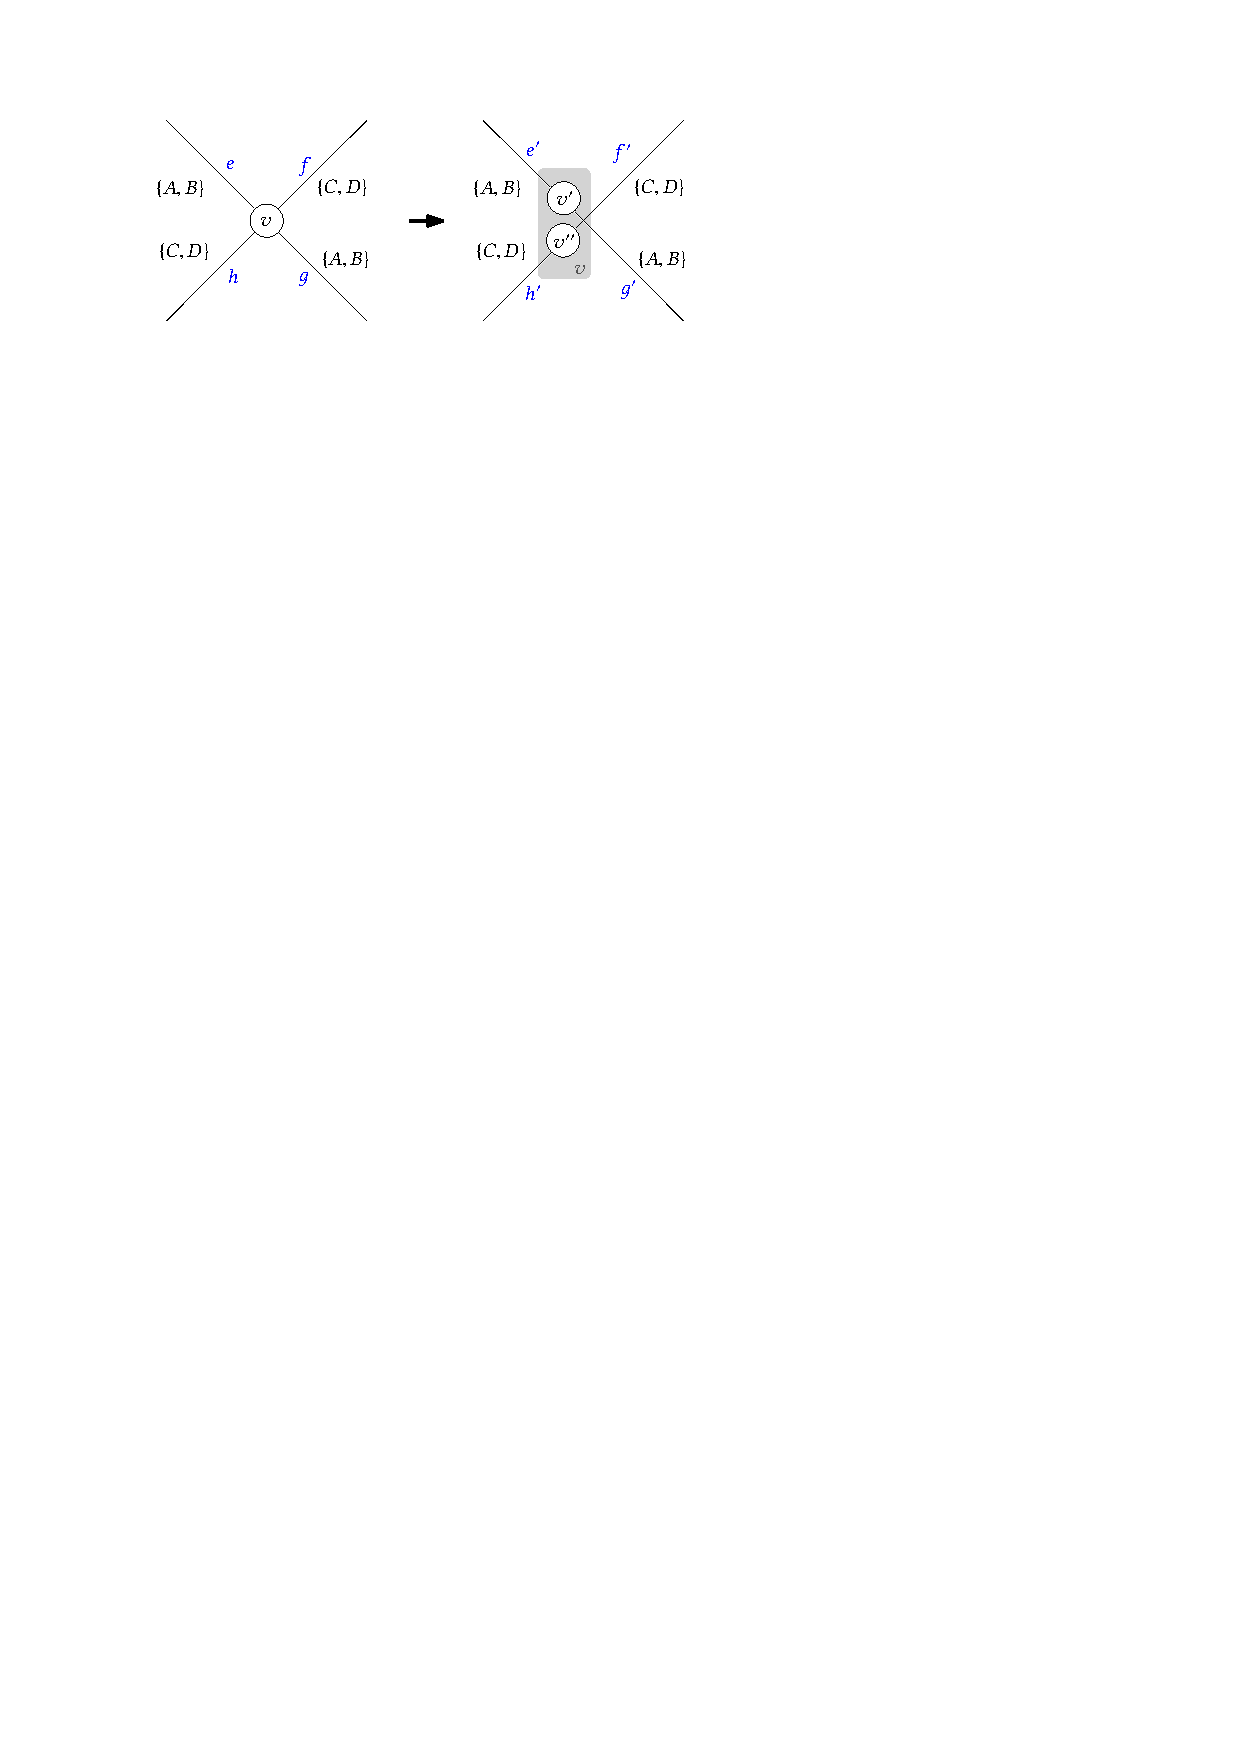
\includegraphics[width=0.68\textwidth]{untangling/fullcross.pdf}
  \caption{Left: Full cross situation in a line graph. $\{A, B\}$ continue from $e$ to $f$ through node $v$ without interfering with $\{C, D\}$ on $h$ and $f$. Right: Node $v$ has been split into two nodes $v'$ and $v''$, without affecting line ordering optimality.}  
  \label{FIG:untangle_fullcross}
  %\vspace{-0.4cm}
\end{figure}

We now consider the situation in Figure~\ref{FIG:untangle_fullcross}, left. It is easy to see that if in some node $v$ we can identify a pair $\{e, f\}$ of adjacent edges with $L(e) = L(f)$, and if neither $e$ or $f$ (partially) continue over into another adjacent edge, the orderings in $e$ and $f$ cannot affect the number of crossing between any $l \in L(e)$ and any $l' \not\in L(e)$, only the number of crossings between themselves. We can thus state the following untangling rule:
\begin{enumerate}[parsep=0.5mm, wide, labelwidth=0mm, itemindent=2.3mm]
  \setlength\itemsep{1pt}
  \item[\emph{(Untangling rule 1)}] For some node $v$ in the line graph and its adjacent edges $e_1, e_2, ..., e_{\deg(v)-1}$, if we can identify two edges $e_a = \{v, u\}$ and $e_b = \{v, w\}$ with $L(e_a) = L(e_b)$ and both $e_a$ and $e_b$ do not (partially) continue into any other edge $e_i \not\in \{e_a, e_b\}$, break $v$ into two nodes $v'$ and $v''$. Node $v'$ gets connected to $u$ with an edge $e'_a$ and to $w$ via $e'_b$, where $L(e'_a) = L(e_a)$ and $L(e'_b) = L(e_b)$. Node $v''$ gets connected to the remaining nodes $u_i$ $v$ was originally connected to via $e'_i = \{v'', u_i\}$. We set $L(e'_i) = L(e_i)$. Figure~\ref{FIG:untangle_fullcross}, right gives an example.
\end{enumerate}

Note that this rule alone will not have any effect on the ILP sizes, as we would for example not add any constraints or variables for crossings between edge $e_a$ and some $e_i \not\in \{e_a, e_b\}$, as described in Sections~\ref{SEC:baseline} and \ref{SEC:improved}. However, $v'$ and $v''$ may now be eligible for contraction according to pruning rule 2a. Additionally, this rule may cause the optimization graph to break down into two connected components.

\subsubsection{Y Structures}

\begin{figure}
  \centering
  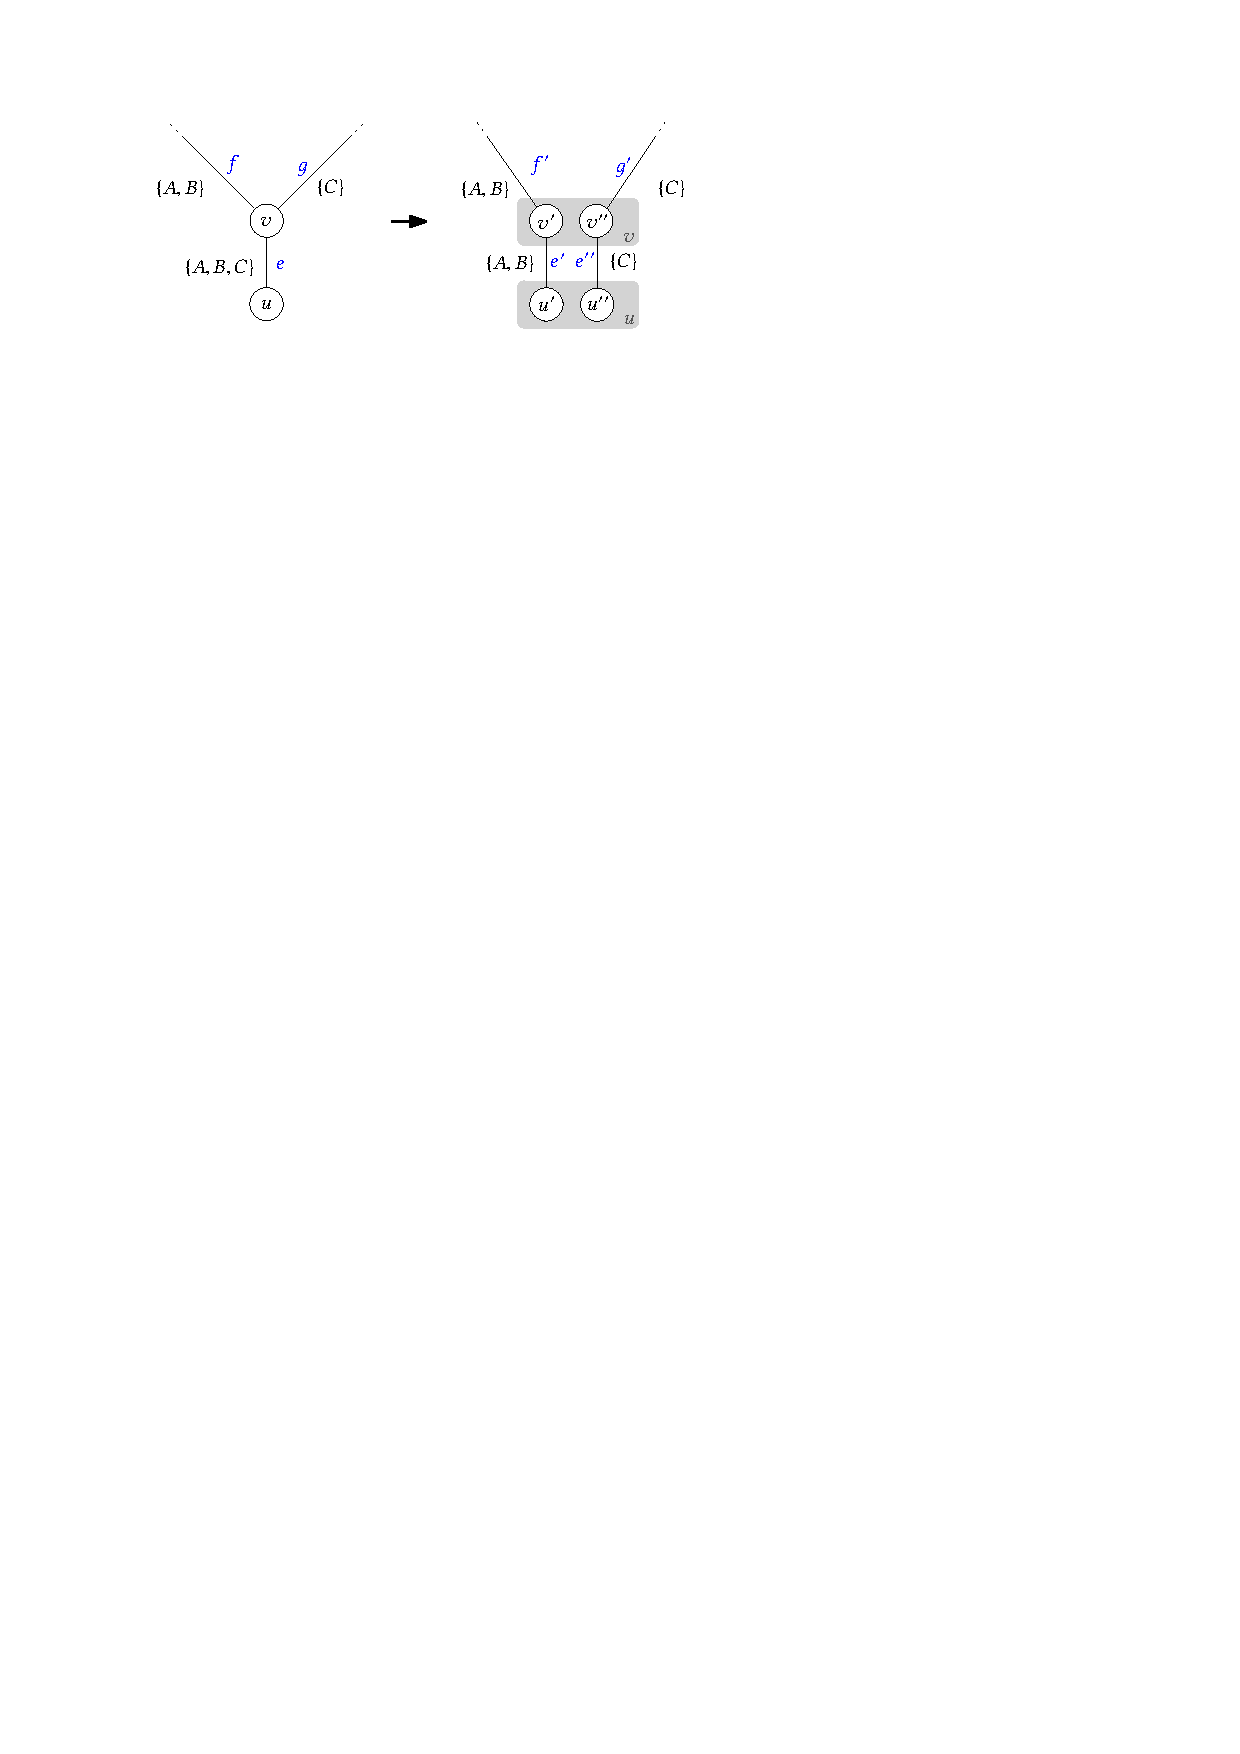
\includegraphics[width=0.68\textwidth]{untangling/y.pdf}
  \caption{Left: TODO. Right: Note that if $g$ was the segment with the largest number of lines in the graph, we now have brought down $M$ from 3 to 2.}  
  \label{FIG:untangle_y}
  %\vspace{-0.4cm}
\end{figure}

Figure~\ref{FIG:untangle_y}, left gives an example of an Y structure in the line graph. Here, a main leg $e = \{u, v\}$ branches at $v$ into two minor legs $f$ and $g$. As $u$ is a terminus, the line ordering in $e$ can always be adjusted to match the line orderings of the minor legs $f$ and $g$ with zero crossings. More specifically, the relative ordering of minor legs $f$ and $g$ already induces a partial optimal ordering of the lines on $e$, namely that $p_e(A) < p_e(C)$ and $p_e(B) < p_e(C)$. Any ordering violating these constraints would induce an unnecessary crossing (or separation) in $v$.

For easier notation, we say that $\rho^v_e(f)$ is the clockwise position of $f$ in node $v$, beginning at edge $e$. For example, in Figure~\ref{FIG:untangle_y}, left, $\rho^v_e(f) = 0$ and $\rho^v_e(g) = 1$.
\begin{enumerate}[parsep=0.5mm, wide, labelwidth=0mm, itemindent=2.3mm]
  \setlength\itemsep{1pt}
  \item[\emph{(Untangling rule 2)}] For some node $v$, if we can identify a main leg edge $e = \{v, u\}$ where $u$ is a terminus and which completely branches at $v$ into $\deg(v) - 1$ minor leg edges $e_{0}, e_{1}, ..., e_{\deg(v) - 2}$ such that $L(e_{0}) \cup L(e_{1}) ... \cup L(e_{\deg(v) - 2}) = L(e)$ and all $L(e_{i})$ are pairwise disjoint, split $v$ and $u$ into nodes $v'$, $v''$ and $u'$, $u''$. For simplicity, we assume that the minor leg edges are already sorted in ascending order by their $\rho^v_{e}$ values. Nodes $v'$ and $u'$ are connected with an edge $e'$, where $L(e') = L(e_{b_0})$ (the lines of the leftmost minor leg). Nodes $v''$ and $u''$ are connected with an edge $e''$, where $L(e'') = \bigcup^{\deg(v) - 2}_{i = 1} L(e_{i})$ (the lines of the remaining minor legs to the right). Additionally, $v'$ gets connected to the nodes it was originally connected to via the first minor leg with $e'_{0}$, where $L(e_{0}) = e'_{0}$. Similarly, all remaining branches are re-connected to $v''$ (Fig.~\ref{FIG:untangle_y}, right).
\end{enumerate}

To be able to later deduce the ordering of the original main leg $e$, we additionally store an ordering of the new main leg edges $e'$ and $e''$, which is just the original clockwise ordering of $e_{b_0}$ and the remainder of the minor legs. The ordering of the lines in the original edge $e$ is then just the ordered lines (after optimization) in $e'$, followed by the ordering lines (after optimization) in $e''$.

Note that this rule only untangles the leftmost minor branch and that a repeated application is necessary to completely untangle more than 2 branches.

\subsubsection{Partial Y Structures}\label{SEC:ypartial}

\begin{figure}
  \centering
  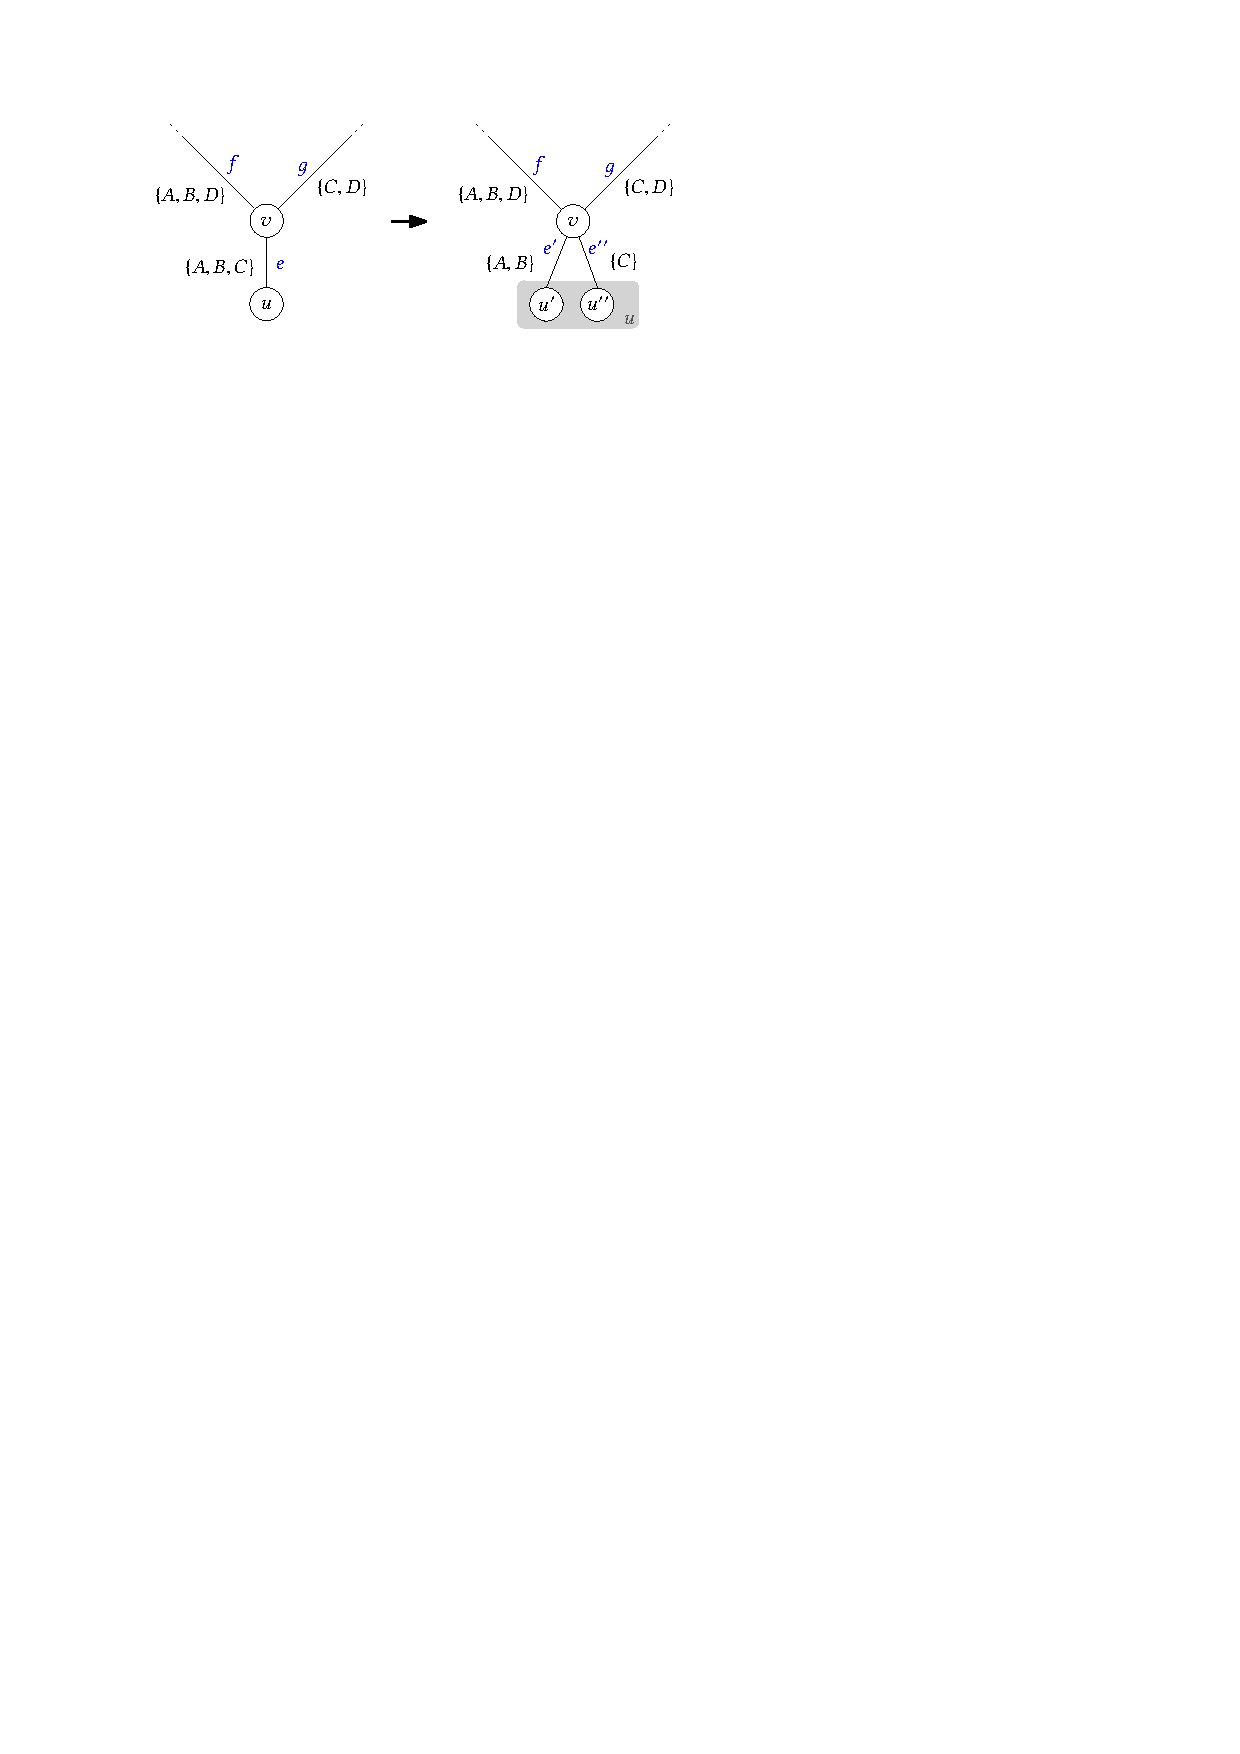
\includegraphics[width=0.68\textwidth]{untangling/y_partial.pdf}
  \caption{Left: Partial Y structure. Right: TODO}  
  \label{FIG:untangle_y_partial}
  %\vspace{-0.4cm}
\end{figure}


A special case of Y structure can be seen in Figure~\ref{FIG:untangle_y_partial}, left. Here, $e$ completely branches into 2 minor legs $f$ and $g$ at $v$. However, the lines of the minor legs are not completely contained in the main leg: line $D$ continues through node $v$ from $f$ to $g$, not to $e$. But the ordering of $f$ and $g$ still induce a partial ordering of $e$. We call this situation a \emph{partial} Y.

\begin{enumerate}[parsep=0.5mm, wide, labelwidth=0mm, itemindent=2.3mm]
  \setlength\itemsep{1pt}
  \item[\emph{(Untangling rule 3)}] For some node $v$, if we can identify a main leg edge $e = \{v, u\}$ where $u$ is a terminus and which completely branches at $v$ into $n$ minor leg edges $e_{0}, e_{1}, ..., e_{n-1}$ such that $L(e_{0}) \cup L(e_{1}) ... \cup L(e_{n-1}) \subsetneq L(e)$, split $u$ into nodes $u'$, $u''$. For simplicity, we again assume that the minor leg edges are already sorted in ascending order by their $\rho^v_e$ values. Similar as in untangling rule 2, $v$ and $u'$ are connected with an edge $e'$, where $L(e') = L(e_{0})$, and $v$ and $u''$ are connected with an edge $e''$, where $L(e'') = \bigcup^{n}_{i = 1} L(e_{i})$  (Fig.~\ref{FIG:untangle_y_partial}, right).
\end{enumerate}

Just like with full Y structures, we store the order of $e'$ and $e''$ to be able to later deduce the line ordering in the original main leg $e$.

\subsubsection{Dog-Bone Structures}\label{SEC:dogbone}

\begin{figure}
\centering
  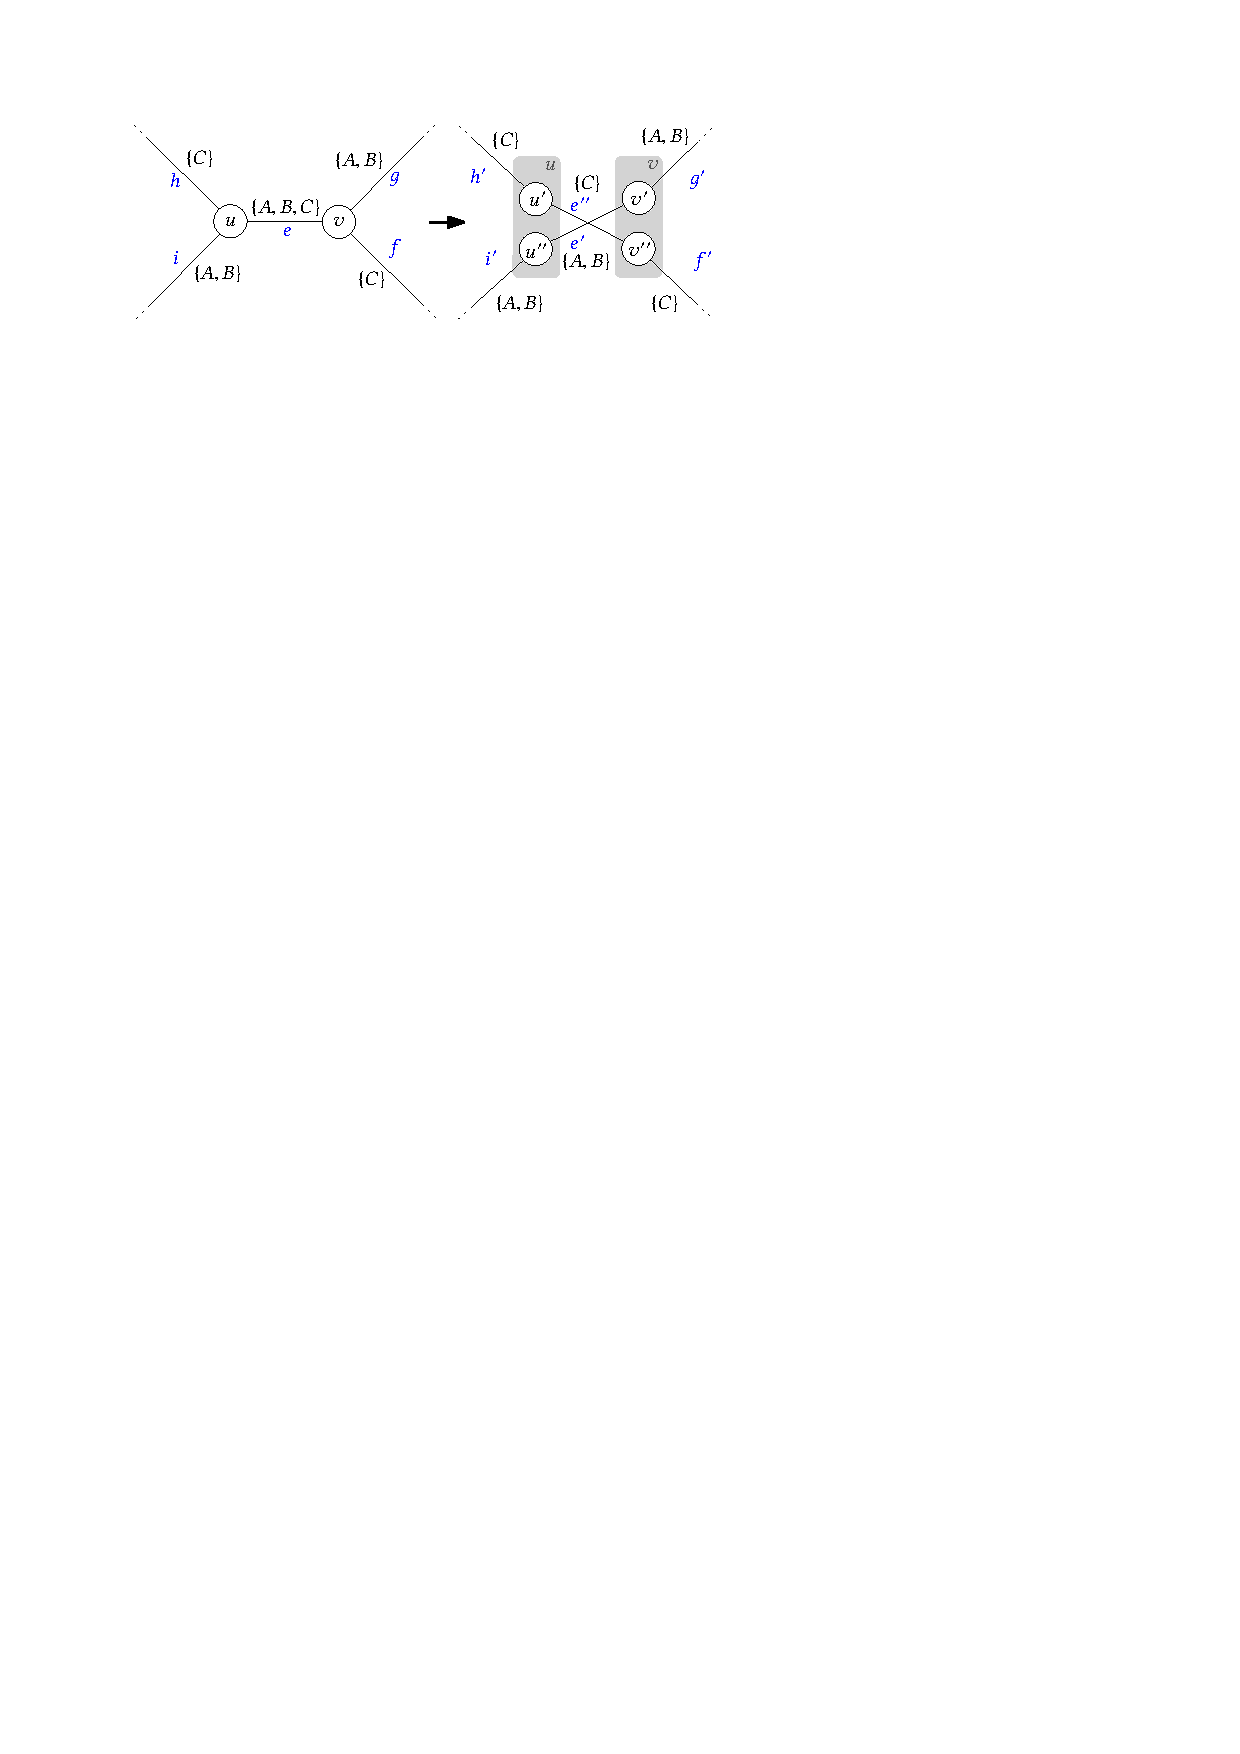
\includegraphics[width=.7\textwidth, page=1]{untangling/dogbone.pdf}
  \caption{Left: TODO. Right: TODO}  
  \label{FIG:untangle_dogbone}

\end{figure}
\begin{figure}
\centering
  \includegraphics[width=.7\textwidth, page=2]{untangling/dogbone.pdf}
  \caption{Left: TODO. Right: TODO}  
  \label{FIG:untangle_dogbone2}
\end{figure}

A more complex structure that is commonly found in real-world input data is depicted in Figure~\ref{FIG:untangle_dogbone}, left. Two line threads (in the example, $\{C\}$ and $\{A, B\}$) on two segments $h$ and $i$ join at some node $u$, continue together for a single segment $e$, and branch again at some node $v$ into $g$ and $f$. We call situations like this dog-bone structures. An example of such a structure in the real-world map of the Stuttgart light rail network is shown in Figure~\ref{FIG:untangle_dogbone_stuttgart}.

\begin{figure}
  \centering
  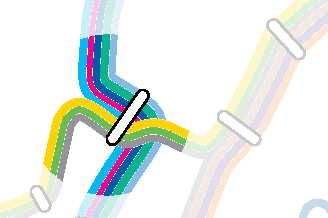
\includegraphics[width=0.49\textwidth, page=1]{untangling/vvs_dogbone.pdf}
  \caption{Dog bone structure in the map of the Stuttgart light rail system. Untangling reduces the number of possible orderings in the highlighted central segment of the network from $8! = 40,320$ to $4! \times 3! = 144$. }  
  \label{FIG:untangle_dogbone_stuttgart}
\end{figure}

Figure~\ref{FIG:untangle_dogbone}, it is obvious to see that there is no reason for $\{C\}$ and $\{A, B\}$ to be intertwined in $e$, for example by setting the ordering on $e$ to $(A, C, B)$: this would only induce an unnecessary splitting between $A$ and $B$, and would not be optimal, regardless of how the rest of the line graph looks like. Additionally, it is also easy to see the ordering of the two threads at $u$ and $v$ imposes a lower bound on the sum of crossings in $u$ and $v$. In Figure~\ref{FIG:untangle_dogbone}, because $\rho^u_e(i) < \rho^u_e(h)$ and $\rho^v_e(g) < \rho^v_e(f)$, two crossings between $C$ and $A$, as well as $C$ and $B$ in either $u$ or $v$ are unavoidable, regardless of the actual orderings in $h$, $i$, $g$ or $f$. In Figure~\ref{FIG:untangle_dogbone_2}, because $\rho^u_e(i) < \rho^u_e(h)$, but $\rho^v_e(f) > \rho^v_e(g)$, no crossing is necessary at all - the two line threads can always continue through $u$ and $v$ next to each other, regardless of their internal ordering. 

We transform structures like this with the following rule:

\begin{enumerate}[parsep=0.5mm, wide, labelwidth=0mm, itemindent=2.3mm]
  \setlength\itemsep{1pt}
  \item[\emph{(Untangling rule 4)}] If some main leg edge $e = (u, v)$, with a degree $\deg(u) = \deg(v) = n \geq 3$ branches at $u$ into $\deg(u) - 1$ minor left leg edges $e^u_{0}, e^u_{1}, ..., e^u_{n}$ and at $v$ into $n$ minor right leg edges $e^v_{0}, e^v_{1}, ..., e^v_{n}$ and if there is a mapping $m(i) \mapsto j$ with $i, j \in [0, n]$ such that $L(e^v_i) = L(e^u_{m(i)})$ ($e$ branches into the exact same left and right branches), we say $e$ is a \emph{dog bone}. We additionally require that $\bigcup^{n}_{i = 0} L(e^u_{i}) = \bigcup^{n}_{j = 0} L(e^v_{j}) = L(e)$ (the combined lines of all left and of all right minor legs are exactly the same as the lines contained in the main leg) and that for both the right and left minor legs, both the $L(e^v_i)$ and the $L(e^u_j)$ are pairwise disjoint (there are no lines continuing through $u$ and $v$ to any other edge than $e$). We then untangle both $u$ and $v$ like $u$ and $v$ in untangling rule 2 (but $u'$ and $u''$ are now also connected to the original left minor leg edges adjacent to $u$) and split $e$ into two edges $e'$ and $e''$, where $e'$ now holds the lines of the first left minor leg, and $e''$ the lines of the remaining minor legs. Figure~\ref{FIG:untangle_dogbone}, right gives an example.
\end{enumerate}

Just like with untangling rule 2 and 3, we have to store an ordering of $e'$ and $e''$ to later deduce the line ordering in the original line graph edge $e$. However, there are now 2 possible orderings we could store: we can either base the ordering of $e'$ and $e''$ on the ordering position of the left minor leg $e^u_0$ in $u$, or on the ordering position of the right minor leg $e^v_0$ in $v$. If the two orderings are inverse, that is if for all $1 \leq i < n$ it holds that $\rho^u_e(e_0) < \rho^u_e(e_i) \Rightarrow \rho^u_e(e_{m(0)}) > \rho^u_e(e_{m(i)})$, it does not matter, because there are no unavoidable crossings we have to consider (Fig.~\ref{FIG:untangle_dogbone2}, right). However, if that is not the case, and an unavoidable crossing occurs (Fig.~\ref{FIG:untangle_dogbone}), right), we have to base the ordering on the node with smaller crossing penalty to not compromise optimality of the final line ordering. For example, in Figure~\ref{FIG:untangle_dogbone}, right, $\rho^u_e(h) > \rho^u_e(i)$. If we assume that $w_\times(u) > w_\times(v)$, we set the ordering of $e'$ and $e''$ in the original line graph edge $e$ to $(e'', e')$, making sure that that after optimization, the ordering in $e$ is either $(C, A, B)$ or $(C, B, A)$, depending on the final ordering of $A$ and $B$. The unavoidable crossings between threads $\{A, B\}$ and $\{C\}$ would then occur in $v$. If $w_\times(u) < w_\times(v)$, the ordering would be set to $(e', e'')$, and the crossings would appear in $u$.

\subsubsection{Partial Dog-Bone Structures}

\begin{figure}
  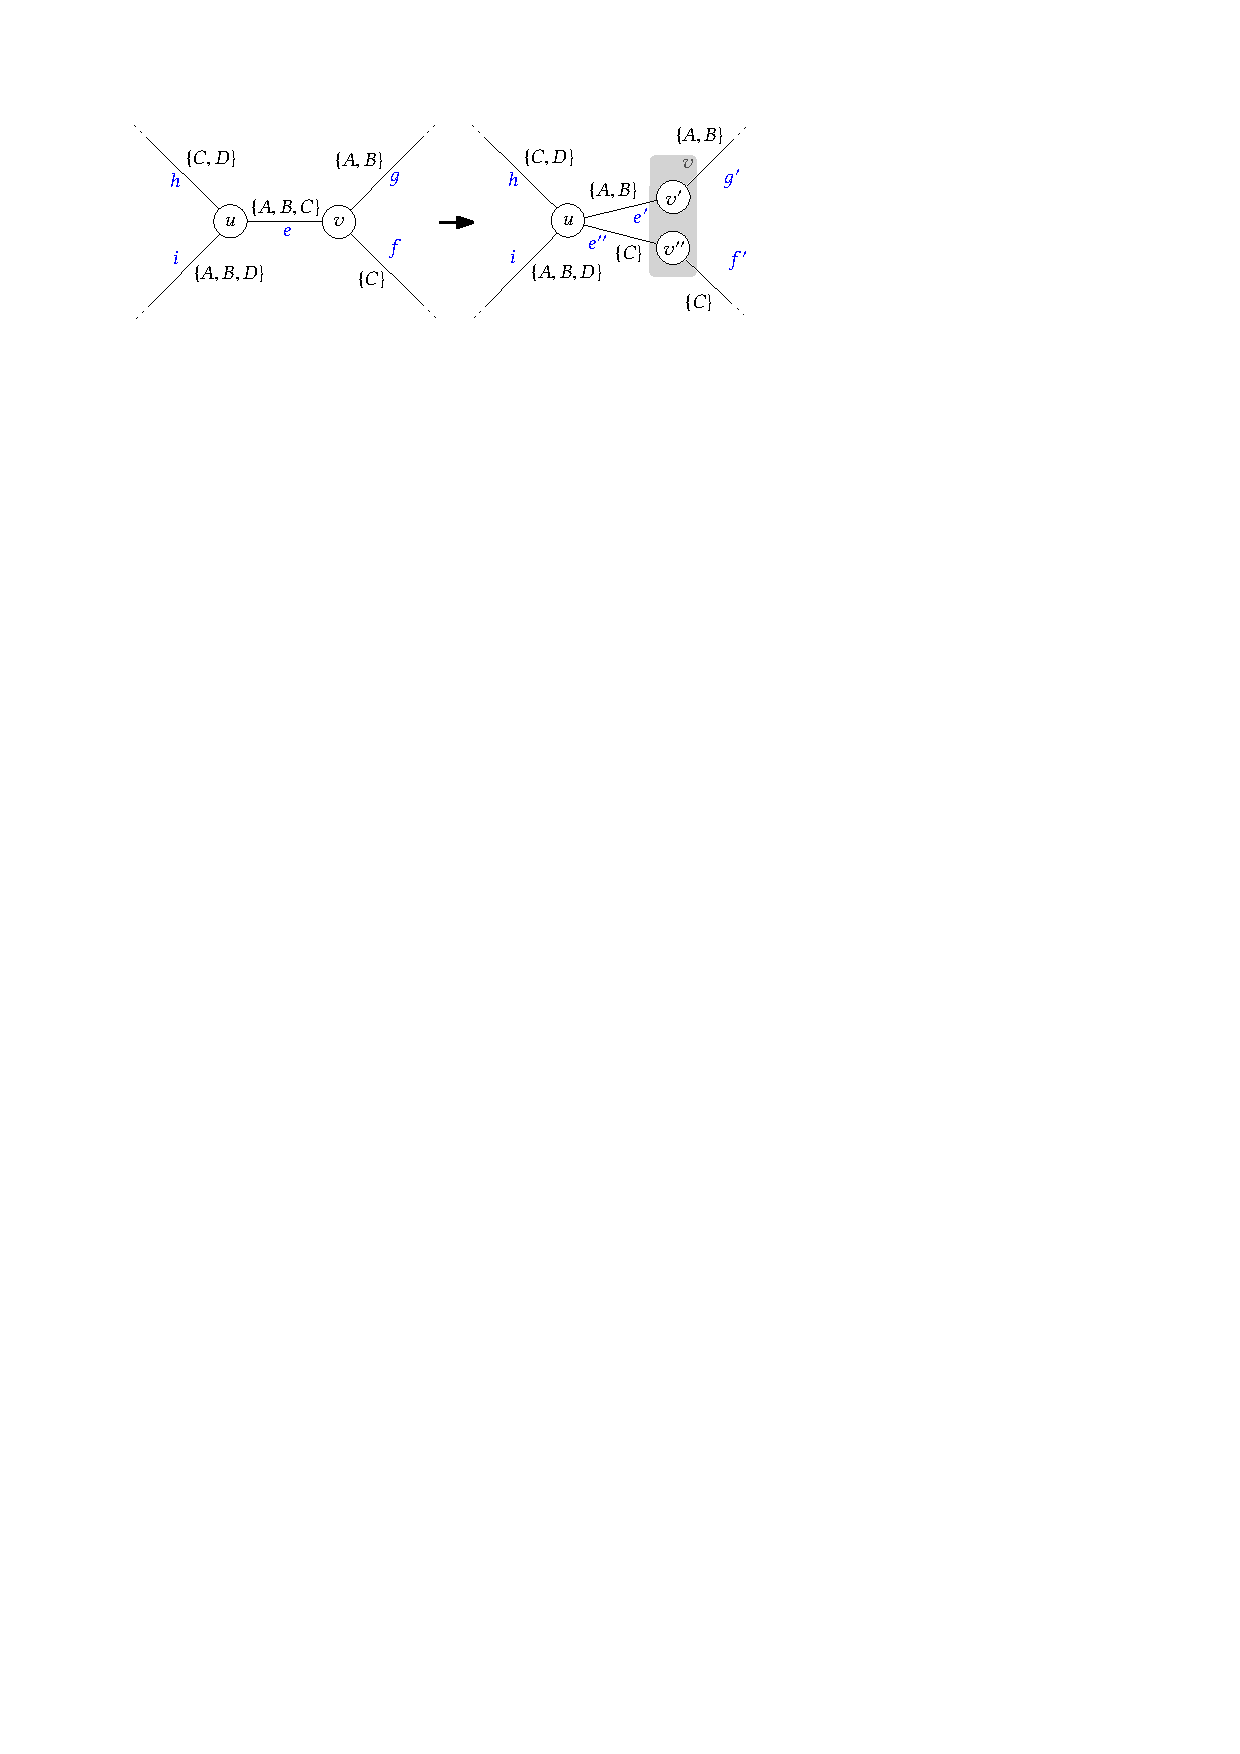
\includegraphics[width=0.7\textwidth, page=1]{untangling/dogbone_partial.pdf}
  \caption{Left: Partial dog bone structure. Right: TODO}  
  \label{FIG:untangle_dogbone_partial}
\end{figure}

For completeness, we note that just as with Y structures, there may also be partial dog-bone structures (Fig.~\ref{FIG:untangle_dogbone_partial}, left). These are dog-bone structures where \emph{one} of the nodes $u$ and $v$ fullfills the criteria described in Section~\ref{SEC:dogbone}, and the other node fullfills the criteria described for $v$ in partial Y structures (Sec.~\ref{SEC:ypartial}) (that is, the main leg branches at $v$ into the same minor legs as at $u$, but $v$ may have additional edges or lines on the minor legs that are not contained in the main leg). 
\begin{enumerate}[parsep=0.5mm, wide, labelwidth=0mm, itemindent=2.3mm]
  \setlength\itemsep{1pt}
  \item[\emph{(Untangling rule 6)}] In cases like the one described above, we only break up the node fullfilling the criteria described in Section~\ref{SEC:dogbone}, just like we broke up only $u$ in Section~\ref{SEC:ypartial} (Fig.~\ref{FIG:untangle_dogbone_partial}, right). By applying untangling rule 4 afterwards, we can then detach the stump line from the main leg.
\end{enumerate}

\subsubsection{Stump Structures}

\begin{figure}
  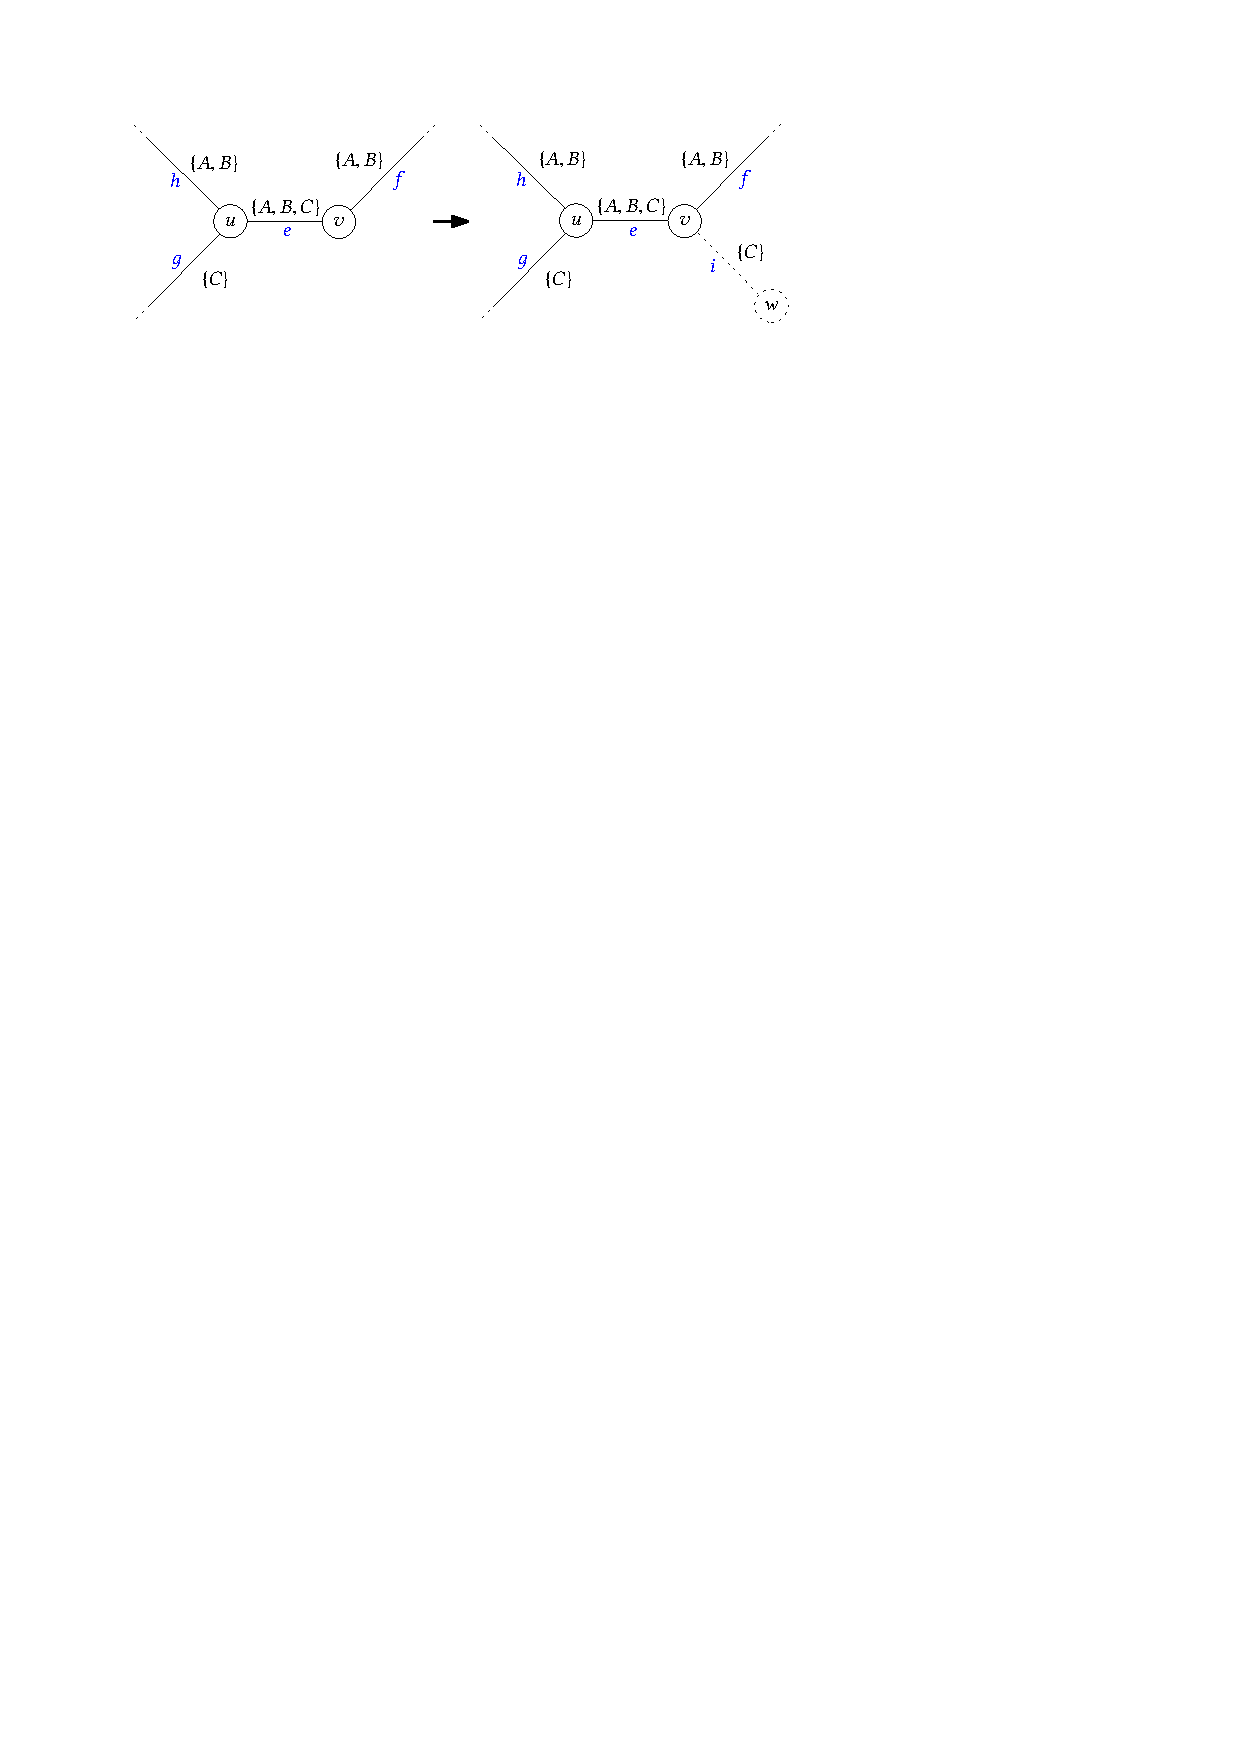
\includegraphics[width=0.7\textwidth, page=1]{untangling/stump.pdf}
  \caption{Left: Stump structure. Right: Stump structure transformed into dog bone.}  
  \label{FIG:untangle_stump}
\end{figure}

It remains to show that an additional class of structures, which we call \emph{stumps}, can be transformed into a dog bone structure with minimal changes to the graph. Figure \ref{FIG:untangle_stump}, left gives an example. Line $C$ on minor leg $g$ attaches itself to the main leg $e$ in node $u$, but already terminates in node $v$, $\{C\}$ is a stump in $e$. Regardless of the ordering of $A$ and $B$ in $h$, $e$ and $f$, the optimal ordering in $e$ is either $(A, B, C)$, or $(B, A, C)$, because we can always put $C$ at the `bottom' of $e$ without introducing a line crossing or a line separation.
\begin{enumerate}[parsep=0.5mm, wide, labelwidth=0mm, itemindent=2.3mm]
  \setlength\itemsep{1pt}
  \item[\emph{(Untangling rule 6)}]We can easily transform a situation like this into a standard dog bone by introducing an additional dummy edge $i$ with the same lines as $g$ from $v$ to an additional dummy node $w$ in such a way that $\rho^v_e(i) = \deg(u) - 1 - \rho^u_e(g)$ ($i$ will be at a position in $v$ that is inverse to the position of $g$ in $u$). 
\end{enumerate}

\subsection{Complexity of Core Graph Reduction}

The real power of the untangling rules described in the previous section lies in their repeated application, together with the pruning and cutting rules described in Sections~\ref{SEC:pruning} and \ref{SEC:cutting}. But how long does it take until an input line graph is fully untangled and reduced?

We first consider the complexity of the untangling rules and assume that the lines in each $L(e)$ are already ordered (for example, by some internal line id). We denote the maximum degree of our input line graph $G$ as $D$. We can safely remove nodes with degree 1 from the line graph prior to optimization and thus assume that $2|E|$ is an upper bound for $|V|$. Finding an edge eligible for any of the untangling rules described in Section~\ref{SEC:untangling} is a matter of iterating over all edges or all nodes, an thus always takes $\mathcal{O}(|E|)$. Each rule breaks up an edge $e$ into two edges $e'$ and $e''$, which can only be done at most $M$ times in the worst case (if $|L(e)| = M$ and we only detach a single line per untangling rule application). No untangling rule increases the number of lines per edge, so a single untangling rule can be applied at most $\mathcal{O}(|E|M)$ times.

In untangling rule 1 (full crossings), we have to check ${D \choose 2} < D^2$ partners of adjacent edges for line equivalency in the worst case, which can always be done in $\mathcal{O}(M)$ because we assume the $L(e)$ to be ordered.

%Applying untangling rule 1 to the entire graph thus takes $\mathcal{O}(|E|M^2D^2)$.

In untangling rule 2 (Y structures), we have to check for the non-terminus node if the $L(e)$ of all minor leg edges are completely contained in the main leg, which can be done in $\mathcal{O}(MD)$, again assuming the $L(e)$ are ordered. We also have to check of the minor leg edges are pairwise disjoint, which takes $\mathcal{O}(MD^2)$ in the worst case. 

%Applying untangling rule 2 to the entire graph thus also takes $\mathcal{O}(|E|M^2D^2)$. Untangling rule 3 makes the same checks as 3, and has thus the same complexity.

In untangling rule 4 and 5 (dog bone structures), it is easy to see that we have to apply the same checks as for rules 2 and 3, but we also have to establish the mapping $m$ between the left and the right legs, which can be considered an intersection problem and solved in $\mathcal{O}(M\Delta(G))$ if we assume that the adjacency lists are already ordered in clockwise fashion based on their outgoing angle.

Untangling rule 6 (stump structures) has the same complexity as rule 4 and 5, as the identification has the same complexity as there and the extension by dummy node and edge can be done in constant time.

A single round of each untangling rule can thus always be done in $\mathcal{O}(|E|MD^2)$.

Now we consider the complexity of the pruning rules. For each contraction, we have to check if $L(e) = L(e')$, which can be solved in $\mathcal{O}(M)$ as we assumed that $L(e)$ and $L(e')$ are sorted and can at least have size $M$. Pruning rule 1 can thus be applied in $\mathcal{O}(|E|M)$, as we have to contract at most $2|E|$ nodes. Pruning rule 2 is a matter of doing at most ${M \choose 2} < M^2$ depth-first searches in the line graph, which can be done in $\mathcal{O}(|E|M^2)$ (again assuming $2|E|$ as an upper bound for $|V|$). Pruning rule 3 is a matter of checking each line in each edge $(u, v)$ if it terminates in either $u$ or $v$, which can again be done in $\mathcal{O}(|E|M)$ as we have to check at least $M$ lines per edges, twice (for $u$ and $v$).

The complexity of cutting rule 1 is trivially $\mathcal{O}(|E|)$, and for cutting rule 2 we have to again check every line in every edge, which can be done in $\mathcal{O}(|E|M)$.

We may apply all of the rules in the following fashion:

\begin{enumerate}
  \item Set n to M.
  \item Apply pruning rule 2 (collapsing of line partners).
  \item Set n to n - 1
  \item Apply pruning rule 1 and 3, apply all cutting rules.
  \item Apply untangling rules 1 - 6.
  \item While n > 0, goto 3.
  \item Apply pruning rule 1 and 3, apply all cutting rules.
\end{enumerate}

First, we note that no cutting, no pruning and no untangling rules increase the number of lines in any edge, so pruning rule 2 has to be applied only once at the beginning.

Second, we note that pruning rule 1 and 3 always \emph{decrease} the number of edges. In the worst case, the cutting rules may double the number of edges. The untangling rules may increase the number of edge by a factor of $M$ in the worst case, so if $|E|$ is the number of edges in the input line graph, the maximum number of edges $|E'|$ in any intermediate optimization graph will be $\mathcal{O}(|E|M)$. We assumed that each edge $L(e)$ and each adjacency list in the input line graph was sorted. The former can be sorted in $\mathcal{O}(|E|M\log M)$, the latter in $\mathcal{O}(|E|D\log D)$.

The worst case complexity of the entire core graph reduction process, including untangling is thus $\mathcal{O}(|E|M^3D^2)$. We note, however, that in practice, both $M$ and $D$ are usually very small. For our testing datasets, the maximum $M$ was 9 (Table~\ref{TBL:datasets}), and $D$ was always below 10. For all practical purposes, we are confident that both $D$ and $M$ can be considered a constant factor.

%
\section{Rendering}\label{SEC:rendering}
%
\begin{figure}[b]
  \centering
  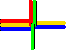
\includegraphics[width=0.35\textwidth]{render_examples/rendering/render_example1.pdf}
  \hspace{1cm}
  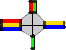
\includegraphics[width=0.35\textwidth]{render_examples/rendering/render_example2.pdf}

  \vspace{0.8cm}
  \centering
  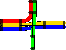
\includegraphics[width=0.35\textwidth]{render_examples/rendering/render_example3.pdf}
  \hspace{1cm}
  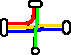
\includegraphics[width=0.35\textwidth]{render_examples/rendering/render_example4.pdf}

	\caption{The four steps of rendering a given line graph: (1) render ordered lines as edges, (2) free node area, (3) render inner connections, (4) render station overlays.}
	\label{FIG:renderingproc}
\end{figure}
This section describes stage 3 of LOOM: given the line graph as computed in stage 1, and a line ordering for each edge as computed in stage 2, render the actual map.
We split this into four basic steps, as illustrated in Fig.~\ref{FIG:renderingproc}.

In the first step (1), a basic skeleton of the map is rendered. We make use of the fact that only a single ordering is imposed on each $L(e)$ and draw each $l \in L(e)$ by perpendicular offsetting the segment's geometry $\tau_{e}$ by $-w\left|L(e)\right|/2 + w\left(p_{e}(l)-1\right)$, where $w$ is the desired line width. As $\tau_{e}$ is just a piecewise linear curve, any method for offsetting (open) polygons may be used. Each drawn node $v$ now has $\deg(v)$ node fronts (Fig.~\ref{FIG:renderingproc}.2). The width of each node front depends on the number of lines on the incident edge and on the the line width $w$. 

In the next step (2), we make room for the line connections between these node fronts by expanding them. As a stopping criteria for this expansion, we simply use a maximum distance from the node front to its original position. 

In a third step (3), the line connections in the node are then rendered by connecting all port pairs (3). In our experiments, we used cubic B\'ezier curves for this, but for schematic maps a circular arc or even a straight line might be preferable.

In the last step (4), we render the stations. This is trivial for nodes of degree $1$ and $2$, but more complicated in large stations with multiple lines. We found that the buffered node polygon already yields reasonable results here, although with much potential for improvement. We also experimented with rotating rectangles until the total sum of the deviations between each node front orientation and the orientation of the rectangle was minimized. Both approaches can be seen in Fig.~\ref{FIG:transitgraphvvs}.

\subsection{Station Merging}

\TODO{This was asked during the conference: what if stations touch during expansion? MERGE THEM}

\section{Evaluation}\label{SEC:eval}
%
\def\degv{\text{deg}(v)}
\def\Hms{\makebox[1.6mm][l]{\hspace{0.2mm}\footnotesize ms}}
\def\Hs{\makebox[1.6mm][l]{\hspace{0.2mm}\footnotesize s}}
\def\Hk{\makebox[1.6mm][l]{\hspace{0.2mm}\footnotesize k}}
\def\Hm{\makebox[1.6mm][l]{\hspace{0.2mm}\footnotesize m}}
\def\Hh{\makebox[1.6mm][l]{\hspace{0.2mm}\footnotesize h}}
\def\Hhline{\\[.7mm]\hline}
We tested LOOM on the public transit schedules of six cities in Europe and the US: Freiburg, Dallas, Chicago, Stuttgart, Turin and New York.
Table~\ref{TBL:datasets} provides the dimensions of each dataset and the time needed to extract the line graph.

\begin{table}[t]
  \caption[]{Line graph dimensions for our testing datasets with extraction times from GTFS. ${\cal S}$ are the stations, $V$ the graph nodes, $E$ the graph edges and ${\cal L}$ the transit lines. $M$ is the maximum number of lines per edge.\label{TBL:datasets}}
  \centering
  %\footnotesize
  {\renewcommand{\baselinestretch}{1.13}\normalsize
  \setlength\tabcolsep{3pt}
  \begin{tabular*}{0.48\textwidth}{@{\extracolsep{\fill}} l r r r r r r} \toprule
              & $t_{\text{extr}}$ & $|{\cal S}|$ & $|V|$ & $|E|$ & $|{\cal L}|$ & $M$ \\\midrule
    Freiburg    & 0.7\Hs  & 74  &  80 &  81 &  5 & 4 \\
    Dallas & 3\Hs & 108 & 117 & 118 &  7 & 4  \\
    Chicago & 13.5\Hs & 143 & 153 & 154 &  8 & 6 \\
    Stuttgart   & 7.7\Hs  & 192 & 219 & 229 & 15 & 8  \\
    Turin       & 4.9\Hs & 339  & 398 & 435 & 14 & 5  \\
    New York
                        & 3.7\Hs & 456  &  517  & 548 & 26 & 9 \\\bottomrule
  \end{tabular*}}

\end{table}
%
\begin{table}[t]
  \caption[]{Core graph dimensions for our testing datasets after applying pruning rules.\label{TBL:datasetscore}}
  \centering
  %\footnotesize
  {\renewcommand{\baselinestretch}{1.13}\normalsize
  \setlength\tabcolsep{3pt}
  \begin{tabular*}{0.48\textwidth}{@{\extracolsep{\fill}} l r r r r r}\toprule
               & $|V|$ & $|E|$ & $|{\cal L}|$ & $M$ \\\midrule
    Freiburg    & 20  & 21  &   5 & 4 \\
    Dallas & 24  & 24  &   7 & 4 \\
    Chicago & 23  & 24  &   8 & 6 \\
    Stuttgart   & 50  & 58  &  15 & 8 \\
    Turin       & 91  & 124 &  14 & 5 \\
    New York
                        & 110 & 138 &  23 & 9 \\\bottomrule
  \end{tabular*}}
  %\vspace{-2mm}
\end{table}

For each dataset, we considered two versions of the line graph: the baseline graph and the core graph.
For each graph, we considered three ILP variants: the baseline ILP (B), the improved ILP (I) and the improved ILP with added separation penalty (I+S).
For each ILP, we evaluated three solvers: the GNU Linear Programming Kit (GLPK), the COIN-OR CBC solver and gurobi (GU).
As most of the datasets (except Turin) still only had one connected component after applying the splitting rules described in Sect.~\ref{SEC:coreprobgraph}, we did not evaluate their application.

For each node $v$, the penalty for a crossing between edge pairs ($\{A, B\}$ in Fig.~\ref{FIG:crossings}, left) was $4 \cdot \degv$, for other crossings ($\{A, B\}$ in Fig.~\ref{FIG:crossings}, right) it was $\degv$. The line separation penalty was $3\cdot\degv$. We found that these penalties produced nicer maps than a uniform penalty. This would imply $w_{\cal S\times} = 4 \cdot \max_{v\in V} \degv$ and $w_{\cal S\|} = 3 \cdot \max_{v\in V} \degv$. However, we found that moving some crossings or separations to stations with a degree greater than $2$ yielded better looking results. Hence, crossings in $v \in \mathcal{S}$ were punished with $w_{\cal S\times}$ if $\degv = 2$ and otherwise with $3\cdot\degv$ (normal crossing) or $12\cdot\degv$ (edge-pair crossing). Similarly, in-station line separations where punished with $w_{\cal S\|}$ if $\degv = 2$ and $9\cdot\degv$ otherwise. Note that Lemma~\ref{LEM:crossingmoveing} still holds because we did not change the punishment for degree 2 stations. Also note that separations were only considered in (I+S) and thus depended on the solver and the input order in (B) and (I).


\begin{figure*}
\centering
%\vspace{1em}
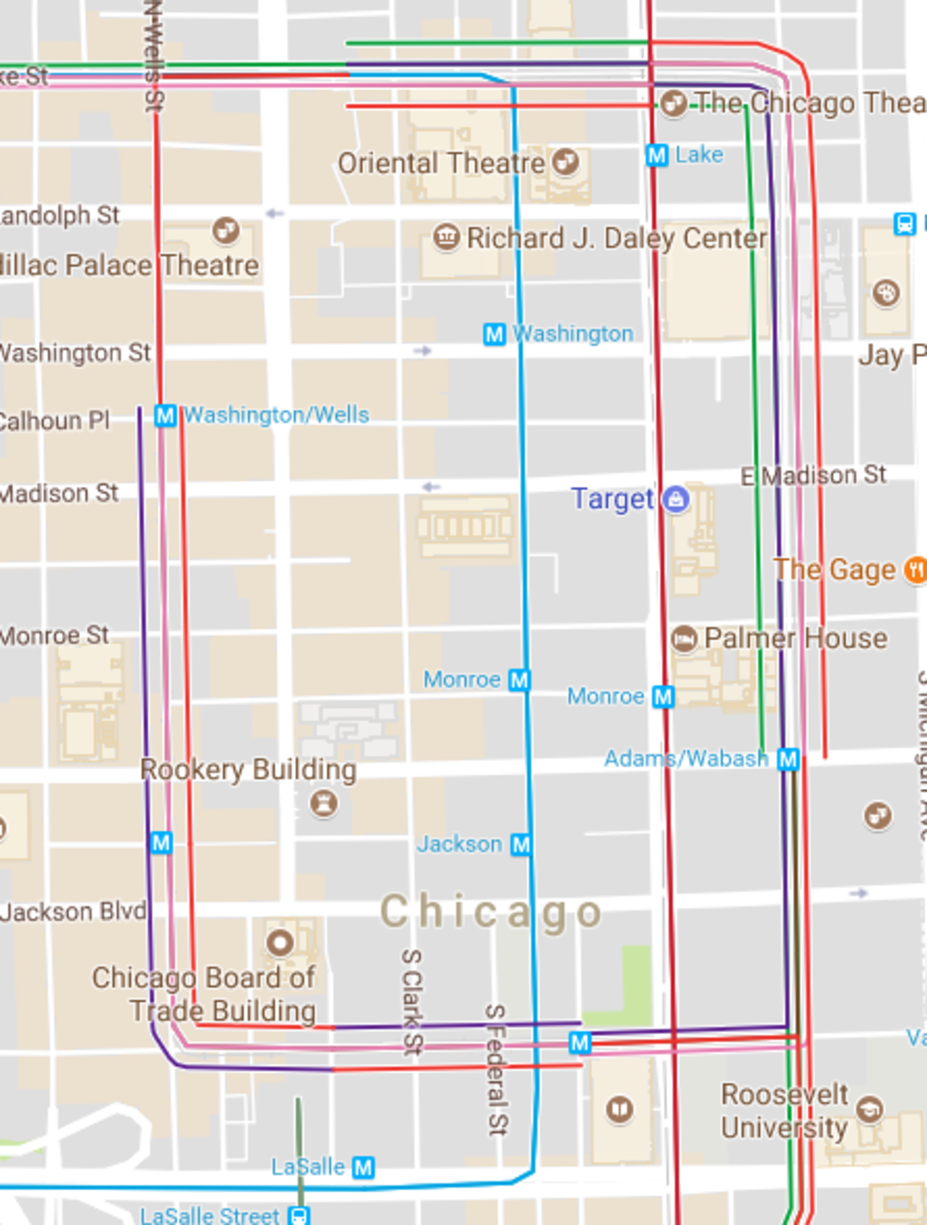
\includegraphics[width=0.32\textwidth]{google.pdf}
\hfill
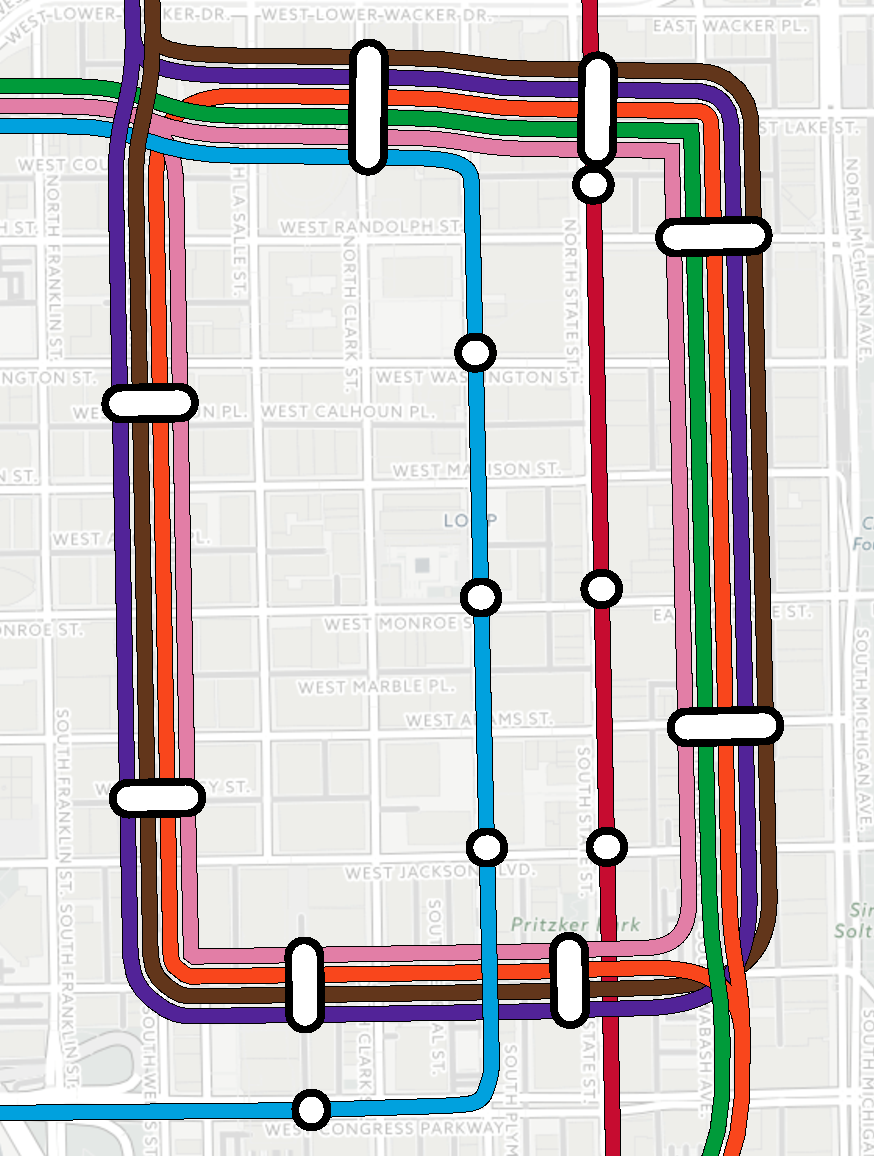
\includegraphics[width=0.32\textwidth]{loom.pdf}
\hfill
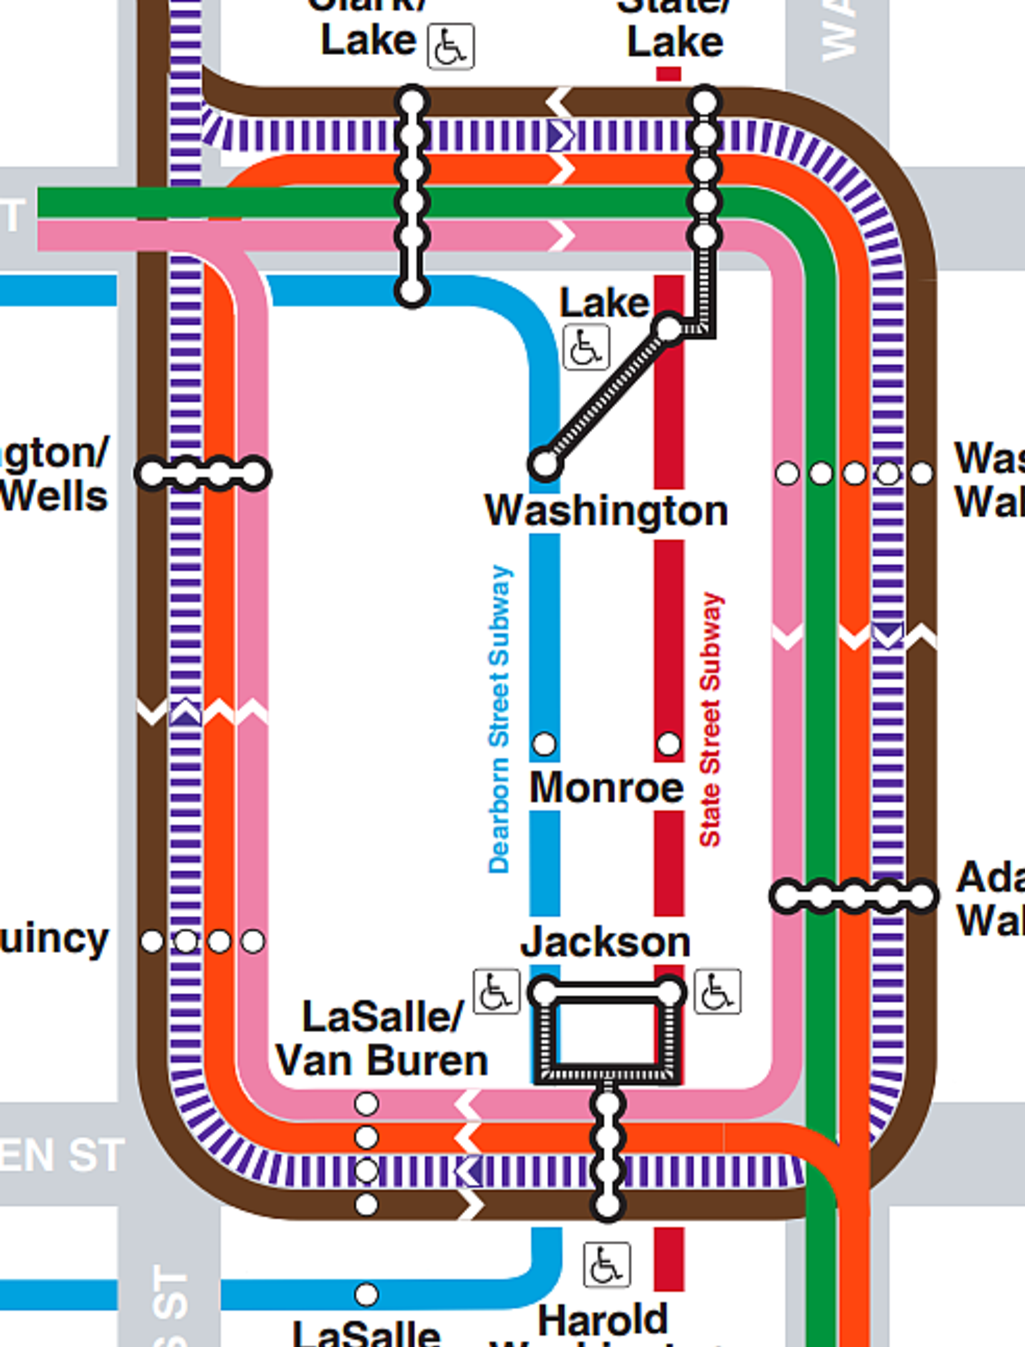
\includegraphics[width=0.32\textwidth]{chicago_loop.pdf}
\caption{Left: Google transit map cutout for Chicago. Center: Same area in our automatically generated map. Right: Official CTA map for the same area. Note the near-perfect match of the line orderings in the official map and our map.}
%\vspace{-1em}
\label{FIG:chicagofull}  
\end{figure*}


\subsection{Performance of Optimization Heuristics}

\TODO{Same table as table 4, but with exhaustive search, hillclimbing and simulated annealing}

\subsection{Comparison of ILP Variants}

Table~\ref{TBL:evalres} shows the results of the ordering optimizations for 4 of our 6 datasets: Chicago, Stuttgart, Turin and New York. Tests were run on an Intel Core i5-6300U machine with 4 cores \`{a} 2.4 GHz and 12 GB RAM.
The CBC solver was compiled with multithreading support, and used with the default parameters and \texttt{threads=4}.
The GLPK solver was used with the feasibility pump heuristic (\texttt{fp\_heur=ON}), the proximity search heuristic (\texttt{ps\_heur=ON}) and the presolver enabled (\texttt{presolve=ON}). We used gurobi with the default parameters.
\subsubsection{ILP Solution Times} With our improved ILP (I), the optimal orderings on the core graph could be found in under 50 milliseconds with gurobi, and in under 1 second with CBC, on any dataset. If line separation was also punished (I+S), the ILP could be solved on the core graph in under 2.5 seconds with gurobi for any dataset, and in under 1 minute with CBC. Although the ILPs for (I+S) were only slightly larger than for (I), optimization on the core graph took $28$ times longer on average with the fastest solver.
\subsubsection{Effects of Core Graph Reduction} On the baseline graph, (B) could not be optimized for all datasets except Turin with gurobi, and only after core graph reduction was a solution for Stuttgart and Chicago found in under 12 hours. As expected in Sect.~\ref{SEC:coreprobgraph}, core graph reduction made the ILPs significantly smaller. On average, the number of rows decreased by $61\,\%$ and the number of columns by $59\,\%$ for (I). For (I+S), the decrease was $62\,\%$ and $60\,\%$, respectively. With the fastest solver and the improved ILP (I), core graph reduction lead to speedup by a factor between $4$ for Chicago, and 2 for New York. For (I+S), this speedup was between $22.4$ for Stuttgart, and $2.5$ for Turin.

\subsection{Impact of Graph Untangling}

\TODO{New table for graph untangling, for all methods and all solvers}

\subsection{Comparison to Manually Designed Maps}

\begin{table}
  \caption[]{Comparison of the line orderings in our maps and in manually designed official maps published by transportation authorities. For the official maps, we hand-counted the number of crossings ($\times$) and separations ($||$) and calculated the score in our penalty system. $T$ is the number of line swaps necessary to transform the line orderings in our map into those of the official map. Swaps between the same two lines on consecutive edges were only counted once. \label{TBL:rweval}}
  \vspace{-3mm}
  \centering
  %\footnotesize
  {\renewcommand{\baselinestretch}{1.13}\normalsize
  \setlength\tabcolsep{3pt}
  \begin{tabular*}{.48\textwidth}{@{\extracolsep{\fill}} l r r r r r r r}
              & \multicolumn{3}{ c }{\footnotesize Official map} & \multicolumn{3}{ c }{\footnotesize Our map} \\
              \cline{2-4} \cline{5-7} \\[-2ex] \toprule\noalign{\smallskip}
              & $\times$ & $||$ & pen. & $\times$ & $||$ & pen. & $T$  \\\midrule
    Freiburg    & 7  & 1  & 132 & 7  &  0 & 48 & 2\\
    Dallas   & 3  & 1  & 27 &  3  &  0 & 9 & 1\\
    Chicago    & 26  & 0  & 80 &  27  &  0 & 80 & 1\\
    Stuttgart    & 65  & 5 & 264 &  64  &  2  & 156 & 4 \\\bottomrule
  \end{tabular*}}
  %\vspace{-2mm}
\end{table}

We also did a manual analysis to evaluate the esthetic quality of our work. For our datasets Freiburg, Dallas, Chicago and Stuttgart, we compared our automatically generated maps to the official maps published by the respective transit agencies\footnote{\url{http://loom.informatik.uni-freiburg.de/officialmaps/vag.pdf}\\\url{http://loom.informatik.uni-freiburg.de/officialmaps/dart.pdf}\\\url{http://loom.informatik.uni-freiburg.de/officialmaps/cta.pdf}\\\url{http://loom.informatik.uni-freiburg.de/officialmaps/vvs.pdf}}. These maps are usually highly simplified and only respect the geographical course of a line to a limited extent. However, they still provide valuable ground truth for the line orderings computed by our ILP (Sect.~\ref{SEC:ordering}).

For each official map, we hand-counted the number of line crossings as well as the number of line separations and calculated the overall score in our penalty system. In addition, we counted the number of line swaps $T$ necessary to transform the line ordering of our map into the line ordering of the official map. Line swaps on multiple consecutive edges were only counted once. Fig.~\ref{FIG:chicagofull} gives an example of that: although we have to swap the brown and the purple line on multiple edges between stations to match the official CTA map, we only count a single, consecutive swap. 

For our 4 manually evaluated datasets, we found that a surprisingly low number of line swaps was necessary to transform the line orderings found by our ILP to the line orderings of the official map. Even for the highly complex 2015 Stuttgart map, only 4 line swaps were required. This is strong evidence that our combination of penalizing line crossings and line separations closely models the esthetics of professional, hand-drawn transit maps.

We also found that our maps always scored better or equal in our penalty system than the official maps, and that only minimal changes to the official map (missed by the designers) would be required to improve the readability. The results can be seen in Table~\ref{TBL:rweval}. For Dallas, our ILP found a single (trivial) line swap that prevented a line separation at no cost and lowered the penalty by 66\%. For Chicago, our orderings nearly match the ones in the official map, but our ILP found a solution with one additional crossing, but equivalent score. For Stuttgart, 4 line swaps could reduce both the number of crossings and the number of separations and lower the penalty by nearly 59\%.


\def\Hdimh{rows\hspace{0.3mm}{\scriptsize$\times$}\hspace{0.3mm}cols}
\def\Hdim#1#2{#1\hspace{0.1mm}{\scriptsize$\times$}\hspace{0.1mm}#2}
\def\Hsci#1#2{$#1${\scriptsize$\times$}$10^{#2}$}
\def\Htglpk{GLPK}
\def\Htcbc{CBC}
\def\Htgo{GU}
%\def\Htglpk{$t_\text{\tiny GLPK}$}
%\def\Htcbc{$t_\text{\tiny CBC}$}
\def\Hlong{---\phantom{\Hs}}
\def\Hno{---}
\def\Hgr{$>$}
\renewcommand*{\thefootnote}{\fnsymbol{footnote}}
\begin{table*}
  \caption[]{Dimensions, solution times and final graph scores (pen) for Chicago, Stuttgart, Turin and New York and three baseline heuristics for the line ordering problem: exhaustive search with (E+S) and without (E) separation penalty and, hill climbing with (H+S) and without (H) separation penalty and simulated annealing with (A+S) and without separation penalty (A), all with or without reduction to the core graph. $|S|$ is the search space size, $t$ the solution time. A time of --- means we aborted after 12 hours. The number of iterations is shown in column \emph{iters}, $\times$ is the number of crossings in the optimized graph, $\|$ the number of separations, \emph{pen} is the final graph score. For optimization without separation penalty, the final graph scores only include crossing penalties. Optimal graph scores can be found in Table~\ref{TBL:rweval}. \label{TBL:evalres_heur}}
  \vspace{-3.6mm}
  \centering
  %\footnotesize
  {\renewcommand{\baselinestretch}{1.13}\normalsize
    \setlength\tabcolsep{2pt}
  \begin{tabular*}{\textwidth}{@{\extracolsep{\fill}} l@{\hskip 1.2mm} c r r r@{\hskip 2.5mm} r r r r r@{\hskip 1.5mm}r@{\hskip 1mm}r r r r}
              && \multicolumn{6}{c}{\footnotesize On baseline graph} & & \multicolumn{6}{c}{\footnotesize On core graph} \\
              \cline{3-8} \cline{10-15} \\[-2ex] \toprule
              && $|S|$ & $t$ & iters & $\times$ & $||$ & pen & & $|S|$ & $t$ & iters & $\times$ & $||$ & pen \\\midrule
    Freiburg    & E & \multirow{6}{*}{\Hsci{6}{13}} & \Hlong & \Hlong & \Hlong & \Hlong & \Hlong & & \multirow{6}{*}{55k} &  4.2\Hs & 55k & 5 & 2 & 42\\
              & H & & 0.2\Hs & 9.5 & 16.9 & 11.2 & 229.9 & &  & 11\Hms & 5.3 & 5.4 & 1.8 & 47.3\\
              & A &  &  90\Hms & 7k & 16.9 & 12.4 & 230.3 & &  & 0.2\Hs & 6.2k & 5.6 & 2 & 49.4\\
              & E+S &  & \Hlong & \Hlong & \Hlong & \Hlong & \Hlong & &  & 5.6\Hs & 55k &  & \Hlong & \Hlong\\
              & H+S &  & 4.3\Hs & 16.9 & 44.6 & 14.3 & 547.2 & &  & 1.1\Hs & 6.9 &  27.3 & 3 & 189.1\\
              & A+S &  &  0.4\Hs & 14.5k & 51.9 & 15.6 & 704.3 & &  & 0.7\Hs & 7.6k & 27.9 & 2.8 & 197.7\\\midrule
    
    Chicago   & E & \multirow{6}{*}{\Hsci{4}{33}} & \Hlong & \Hlong & \Hlong & \Hlong & \Hlong & & \multirow{6}{*}{\Hsci{5}{9}} & \Hlong & \Hlong & \Hlong & \Hlong & \Hlong\\
              & H & & 3\Hs &  16.8 & 48.1 & 38.5 & 592.7 & &  & 1.2\Hs & 7.4 & 25.5 & 8.7 & 182.4\\
              & A &  &  0.2\Hs & 11k & 55.6 & 43.6 & 687.9 & &  & 0.7\Hs & 9k & 25.4 & 9.1 & 183.7\\
              & E+S &  & \Hlong & \Hlong & \Hlong & \Hlong & \Hlong & &  & \Hlong & \Hlong & \Hlong & \Hlong & \Hlong\\
              & H+S &  & 4.3\Hs & 16.9 & 44.6 & 14.3 & 547.2 & &  & 1.1\Hs & 6.9 &  27.3 & 3 & 189.1\\
              & A+S &  &  0.4\Hs & 14.5k & 51.9 & 15.6 & 704.3 & &  & 0.7\Hs & 7.6k & 27.9 & 2.8 & 197.7\\\midrule
  \end{tabular*}}
  \vspace{3.6mm}
\end{table*}

\begin{table*}
  \caption[]{Dimensions and solution times for Chicago, Stuttgart, Turin and New York and our three ILPs: baseline (B), improved (I), and with line separation penalty (I+S), with or without reduction to the core graph, solved with GLPK, COIN-OR CBC and gurobi (GU). A time of --- means we aborted after 12 hours. The last two columns show the number of crossings ($\times$) and separations ($||$) after optimization. Optimal graph scores can be found in Table~\ref{TBL:rweval}.\label{TBL:evalres}}.
  %\vspace{-50mm}
  \centering
  %\footnotesize
  {\renewcommand{\baselinestretch}{1.13}\normalsize
    \setlength\tabcolsep{2pt}
  \begin{tabular*}{\textwidth}{@{\extracolsep{\fill}} l@{\hskip 1.2mm} c r r r@{\hskip 2.5mm} r r r r r@{\hskip 1.5mm}r@{\hskip 1mm}r r r}
              && \multicolumn{4}{c}{\footnotesize On baseline graph} & & \multicolumn{4}{c}{\footnotesize On core graph} \\
              \cline{3-6} \cline{8-11} \\[-2ex] \toprule
              && \Hdimh & \Htglpk & \Htcbc & \Htgo &  & \Hdimh & \Htglpk & \Htcbc & \Htgo & $\times$ & $||$ \\\midrule

    Chicago   & B & \Hdim{41\Hk}{861}   & \Hlong &  \Hlong & \Hlong & &  \Hdim{8.2\Hk}{266} &  \Hlong & 47\Hm & 2\Hm &   22 &   4-7 \\
              & I & \Hdim{1.4\Hk}{982} &  9\Hs & 1\Hs & 41\Hms & &   \Hdim{394}{285} & 0.8\Hs &  0.1\Hs & 10\Hms &   22 &   4-7 \\
              & I+S & \Hdim{1.9\Hk}{1.2\Hk} &  47\Hm &   19\Hs & 1.8\Hs & &   \Hdim{505}{338} &   23\Hs &  3.8\Hs & 0.3\Hs &   27 &     0\\\midrule

    Stuttgart & B & \Hdim{224\Hk}{2.4\Hk} & \Hlong &  \Hlong & \Hlong & &   \Hdim{44\Hk}{950} &  \Hlong &  \Hlong & 10\Hh & 60 &  11 \\
              & I & \Hdim{4.1\Hk}{2.8\Hk} & \Hlong &  3.5\Hs & 0.1\Hs & & \Hdim{1.5\Hk}{1\Hk} &   8\Hs &  0.2\Hs &  36\Hms &  60 & 7-15 \\
              & I+S & \Hdim{5.6\Hk}{3.5\Hk} & \Hlong &  2\Hm & 47\Hs & & \Hdim{2.1\Hk}{1.3\Hk} &  \Hlong &   36\Hs & 2.1\Hs &   64 &     2 \\\midrule

    Turin     & B & \Hdim{24\Hk}{2.1\Hk}  & \Hlong &   \Hlong & 14\Hm & &   \Hdim{13\Hk}{1\Hk}     &  \Hlong  &  \Hlong &2\Hm & 79 & 6  \\
              & I & \Hdim{3.3\Hk}{2.4\Hk}   & 2\Hm & 0.6\Hs   & 0.1\Hs & &   \Hdim{1.6\Hk}{1.1\Hk}  &  16\Hs &  0.3\Hs & 41\Hms &    79     &   6-10\\
              & I+S & \Hdim{4.3\Hk}{2.9\Hk}   & \Hlong  &  14\Hs   & 1\Hs & &   \Hdim{2\Hk}{1.4\Hk} &  \Hlong   &  4.2\Hs & 0.4\Hs &    81     &     2 \\\midrule

    New York  & B & \Hdim{229\Hk}{5.2\Hk} & \Hlong &  \Hlong & \Hlong & &  \Hdim{96\Hk}{2.3\Hk} &  \Hlong &  \Hlong & \Hlong & \Hno &  \Hno \\
              & I &  \Hdim{8.6\Hk}{6\Hk} & \Hlong &  1.8\Hs & 0.2\Hs & & \Hdim{3.7\Hk}{2.5\Hk} &   \Hlong &  0.7\Hs & 0.1\Hs &  127 &     6-14 \\
              & I+S &  \Hdim{12\Hk}{7.4\Hk} & \Hlong &  2.5\Hm & 12\Hs & & \Hdim{4.9\Hk}{3.2\Hk} &  \Hlong &   50\Hs &  1.5\Hs & 132  &     2 \\\bottomrule
  \end{tabular*}}
  %\vspace{50mm}
\end{table*}
  

\section{Conclusions and Future Work}\label{SEC:conclusions}

This paper presented a complete end-to-end method for producing geographically accurate transit maps from raw schedule data. We evaluated LOOM, a full implementation of this method, and showed that it produces geographically accurate transit maps fast. We demonstrated that our intuition of punishing both line crossings and line separations lead to results that closely resemble the esthetics of manually designed maps.

The biggest challenge was getting the optimal line orderings in acceptable time. We have shown that with an improved formulation of our ILP and several pruning and cutting rules we could reduce the solve time by several orders of magnitude for some datasets, compared to our initial approach. The whole pipeline (including line graph construction from GTFS schedule data, line ordering optimization and rendering) took less than 15 seconds for all considered inputs.

It may be interesting to additionally compare our ILP solution times and the final solution scores to a heuristic baseline (for example, a local search).

Since the line graph construction required more time than the subsequent ILP solution for some datasets, faster algorithms for extracting the line graph would help to further decrease the running time. It would be interesting to evaluate the adaptability of other map construction algorithms to this problem, both in terms of running time and quality.

As mentioned in Sect.~\ref{SEC:rendering}, we see room for improvement in the rendering of station polygons. It may be necessary to enforce a local octilinearity on edges leaving stations for a cleaner look. Another open problem is that of overlapping station nodes on very small resolutions.

Both our line-ordering and rendering steps may be used with any multigraph as input and are not restricted to a geographically accurate network. It may be interesting to evaluate LOOM on schematic transit networks as well.

Lastly, the ideas behind LOOM may be useful also in a non-transit scenario.
For example, one closely related problem is that of wire routing in integrated-circuit design.
There, stations correspond to chips and other elements (which in wire routing are indeed of polygonal form), lines correspond to wires, and the geographical course of the lines may correspond to a pre-existing wiring.

%TODO: mention octilinear maps

%\TODO{mention thorough aesthetical evaluation via crowd-sourcing?}
%
%\TODO{mention station rendering, which is sub par atm}
%
%\TODO{mention that transit maps are not only useful for transit, but also to visualize for example flowcharts or storylines, layouts of electronic circuits}
%
%\TODO{maybe mention stability across zoom levels}

\bibliographystyle{ACM-Reference-Format}
\bibliography{transitmaps}

\end{document}
